% TODO ref donnée dans SUM15!!!+poupart+... FACTO PROB/POSS

%% TODO!!! est-ce qu'on a dit qu'on utilisait mixed opt/pess dans les expé du chap updates??

%\subsection{aaai}
%Qualitative Possibilistic Mixed-Observable MDPs ($\pi$-MOMDPs), generalizing
%$\pi$-MDPs and $\pi$-POMDPs, are well-suited models to planning under
%uncertainty with mixed-observability when transition, observation and reward
%functions are not precisely known and can be qualitatively described. 
%Functions defining the model as well as intermediate calculations are 
%valued in a finite possibilistic scale $\mathcal{L}$, which induces
%a \emph{finite} belief state space under partial observability
%contrary to its probabilistic counterpart. 
In this chapter, we propose 
the study of factored $\pi$-MOMDP models 
in order to solve large
structured planning problems 
under qualitative uncertainty, 
or considered
as qualitative approximations of probabilistic problems. 
Building upon the SPUDD
algorithm for solving factored (probabilistic) MDPs, 
we conceived a symbolic
algorithm named PPUDD for solving 
factored $\pi$-MOMDPs. Whereas SPUDD's
decision diagrams' leaves may be 
as large as the state space since their values
are real numbers aggregated through 
additions and multiplications, PPUDD's ones
always remain in the finite scale $\mathcal{L}$ 
via $\min$ and $\max$ operations only.
Finally,
we present a sound transformation from factored
mixed-observable possibilistic problems with both hidden and visible state
variables to fully observable ones, on which PPUDD is run.
Our experiments show that PPUDD's 
computation time is much lower than SPUDD,
Symbolic-HSVI and APPL for possibilistic 
and probabilistic versions of the same
benchmarks under either total 
or mixed-observability, while still providing
high-quality strategies. 

\section{Introduction}
%Many sequential decision-making problems under
%uncertainty can be easily expressed in terms of Markov Decision Processes (MDPs)
%\cite{Bel}. %,Puterman-MDP}. 
%Partially Observable MDPs (POMDPs)
%\cite{Smallwood_Sondik} take into account situations where the system's state is
%not totally visible to the agent. Finally, the Mixed Observable MDP (MOMDP)
%framework \cite{OngShaoHsuWee-IJRR10,AraThoBufCha-ICTAI10} generalizes both
%previous ones by considering that states can be expressed in terms of two parts,
%one visible and the other hidden to the agent, which reduces the dimension of
%the infinite belief space. %it results in a hybrid
% discrete/continuous belief
% MDP.
% Yet,
%these frameworks encounter difficulties in computing
%big state space fully observable MDPs requires lot of time to compute optimal
% policies.
%With regard to POMDPs, exact dynamic programming algorithms like incremental
%pruning \cite{Cassandra97incrementalpruning:} can only solve very small
%problems: many approximation algorithms have been proposed to speed up
%computations while controlling the quality of the resulting policies
%\cite{Pineau_2003_4826,Smith:2004:HSV:1036843.1036906,Kurniawati-RSS08}. In this
%paper, we proceed quite differently: we start with an approximated
%\emph{qualitative} model that we exactly solve.
%Qualitative possibilistic MDPs ($\pi$-MDPs), POMDPs ($\pi$-POMDPs) and more
%broadly MOMDPs ($\pi$-MOMDPs) were introduced in
%\cite{Sabbadin2001287,DBLP:journals/ijar/SabbadinFL98,Sabbadin:1999:pipomdp,Drougard13}.
%These possibilistic counterparts of probabilistic models
%are based on Possibility Theory \cite{DuPr1988.4} and more specifically on
%Qualitative Decision Theory \cite{DBLP:journals/eor/DuboisPS01,Dubois95possibilitytheory}.
%A possibility distribution, classically models imprecision or 
%lack of knowledge about the model. 
%Links between probabilities and possibilities are theoretically well-understood:
As explained at the end of the previous chapter, 
starting from a probabilistic MOMDP \cite{OngShaoHsuWee-IJRR10,AraThoBufCha-ICTAI10},
the use of Possibility Theory instead of Probability Theory 
leads to an approximation of the initial 
probabilistic model \cite{conf/ecai/Sabbadi00}:
probabilities and rewards are replaced by 
qualitative statements that lie in a finite scale 
(as opposed to continuous ranges in the probabilistic framework), 
which results in simpler computations. 
Possibilities and probabilities have similar behaviors for problems with low
entropy probability distributions \cite{Dubois04probability-possibilitytransformations}.
However, the decision resulting from both models 
can be completely different in practice.
Consider for example a situation in which
three actions $a_A$, $a_B$ and $a_C$ 
lead to three different sets of system states:
\begin{itemize}
\item action $a_A$ leads to $\mathcal{S}_A = \set{s_A^1,s_A^2}$, with
$\textbf{p} \paren{ s_A^1 \sachant a_A } = \textbf{p} \paren{ s_A^2 \sachant a_A } = 0.5$,
$r(s_A^1,a_A) = 1$ and $r(s_A^2,a_A) = 0$;
\item action $a_B$ leads to $\mathcal{S}_B = \set{s_B^1}$ 
($\textbf{p} \paren{ s_B^1 \sachant a_B } = 1$)
with $r(s_B^1,a_B) = 0.5$;
\item action $a_C$ leads to $\mathcal{S}_C = \set{s_C^1,\ldots,s_C^7 }$
with $\textbf{p} \paren{ s_C^1 \sachant a_C }=0.4$,
$\textbf{p} \paren{ s_C^2 \sachant a_C }
= \ldots
= \textbf{p} \paren{ s_C^7 \sachant a_C } = 0.1$,
$r(s_C^1,a_C) = 0$ 
and $r(s_C^2,a_C)=\ldots=r(s_C^7,a_C) = 1$.
\end{itemize}
Actions $a_A$ and $a_B$ lead to the same average gain: $0.5$.
However, action $a_C$ leads to a better one: $0.6$.
Now, let us define a possibilistic model respecting the ranking of event plausibilities: 
\begin{itemize}
\item $\pi \paren{ s_A^1 \sachant a_A } = \pi \paren{ s_A^2 \sachant a_A } = 1$,
$\rho(s_A^1,a_A) = 1$ and $\rho(s_A^2,a_A) = 0$;
\item $\pi \paren{ s_B^1 \sachant a_B } = 1$ and $\rho(s_B^1,a_B) = \frac{3}{4}$;
\item $\pi \paren{ s_C^1 \sachant a_C }=\frac{2}{4}$,
$\pi \paren{ s_C^2 \sachant a_C }
= \ldots
= \pi \paren{ s_C^7 \sachant a_C } = \frac{1}{4}$,
$\rho(s_C^1,a_C) = 0$ 
and $\rho(s_C^2,a_C)=\ldots=\rho(s_C^7,a_C) = 1$.
\end{itemize}
The action $a_A$ is chosen by the optimistic approach.
Indeed, it is entirely possible to reach $s_A^1$
($\pi \paren{ s_A^1 \sachant a_A } = 1$)
whose preference is $1$.
The action $a_B$ is chosen by the pessimistic approach
since the preference $\frac{3}{4}$ is reached with certainty
with this action:
action $a_A$ leads potentially to $s_A^1$ with the preference 
$\rho(s_A^2,a_A)=0$, and $a_C$ leads potentially to $s_C^1$
with $\rho(s_C^1,a_C) = 0$.
Thus, in some cases, 
the three approaches, (the optimistic, pessimistic possibilistic approaches 
and the probabilistic approach) 
may select three different actions.

Recall that the possibilistic approach benefits from computations 
on \emph{finite} belief state spaces, 
whereas probabilistic MOMDPs tackle \emph{infinite} ones. 
It means that the same algorithmic techniques can be used to solve $\pi$-MDPs,
$\pi$-POMDPs or $\pi$-MOMDPs. 
What is lost in precision of the uncertainty model is saved 
in computational complexity. Problems where the uncertainty model is
imprecisely known are also are naturally well-modeled by $\pi$-MOMDPs \cite{Drougard13}: 
e.g., occurrence frequencies of observations resulting from a complex
image processing algorithm depend on many environmental factors like lightening
conditions so that they are generally not precisely known.

Previously presented works on $\pi$-(MO)MDPs do not totally take advantage of
the problem structure, i.e. visible or hidden parts of the state can be
themselves factored into many state variables, which are flattened by
current possibilistic approaches. In probabilistic settings, factored MDPs 
and Symbolic Dynamic Programming (SDP) frameworks
\cite{DBLP:journals/ai/BoutilierDG00,Hoey99spudd:stochastic} have been
extensively studied in order to reason directly at the level of state variables
rather than state space in extension.
A more recent work is for instance \cite{DBLP:conf/ecai/RadoszyckiPS14}. 
However, factored probabilistic
MOMDPs have not yet been proposed to the best of our knowledge, probably because
of the intricacy of reasoning with a mixture of a finite state subspace and an
infinite belief state subspace due to the probabilistic model -- contrary to the
possibilistic case where both subspaces are finite. The famous algorithm SPUDD
\cite{Hoey99spudd:stochastic} solves factored probabilistic MDPs by using
symbolic functional representations of value functions and strategies in the form
of Algebraic Decision Diagrams (ADDs) \cite{Bahar:1997:ADD}, which compactly
encode real-valued functions of Boolean variables: ADDs are directed acyclic
graphs whose nodes represent state variables and leaves are the function's
values. Instead of updating state values individually at each iteration of the
algorithm, they are aggregated within ADDs and operations are symbolically and
directly performed on ADDs over many states at once. However, SPUDD suffers from manipulation of
potentially huge ADDs in the worst case: for instance,
expectation involves additions and multiplications of real values (probabilities
and rewards), creating other values in-between, in such a way that the number of
ADD leaves may equal the size of the state space, which is exponential in the
number of state variables.
Therefore, the work presented here is motivated by the simple observation that
\textbf{symbolic operations with possibilistic MDPs would necessarily
limit the size of ADDs}: indeed, this formalism operates over a \emph{finite}
possibilistic scale $\mathcal{L}$ with only $\max$ and $\min$ operations involved,
which implies that all manipulated values remain in the %$\mathcal{L}$ 
%of their leaves would be at most equal to the cardinal of the possibilistic
finite scale $\mathcal{L}$, which is generally far smaller than the number of states.
\begin{figure} \centering
\begin{tikzpicture}
\begin{axis}[grid=major,xmax=100,
legend entries={ $8$ variables: qualitative settings, quantitative settings,  
$10$ variables: qualitative settings, quantitative settings},legend style={at={(2,0.6)}},
xlabel={Size of the scale $\mathcal{L}$},
ylabel={Maximal number of nodes},
title={Maximal number of nodes of an ADD: leaves in $\mathcal{L}$ versus in $\mathbb{R}$}]
\addplot table[x=scaleSize, y=MaxNbNodesPoss]{ADDsizeFctLsize/src/MAXnbNodes_fctOf_Lsize_8VARS.txt};
\addplot table[x=scaleSize, y=MaxNbNodes]{ADDsizeFctLsize/src/MAXnbNodes_fctOf_Lsize_8VARS.txt};
\addplot table[x=scaleSize,y=MaxNbNodesPoss]{ADDsizeFctLsize/src/MAXnbNodes_fctOf_Lsize_10VARS.txt};
\addplot table[x=scaleSize,y=MaxNbNodes]{ADDsizeFctLsize/src/MAXnbNodes_fctOf_Lsize_10VARS.txt};
\end{axis}
\end{tikzpicture}
\caption[Limitations of the maximal size of an ADD in the possibilistic settings]{
The maximal size (total number of nodes) 
of an ADD whose values are in $\mathcal{L}$,
\textit{i.e.} in qualitative settings, is limited:
the upper bound is represented in blue and brown lines with circles,
as a function of the size of $\mathcal{L}$.
When the leaves of the ADD are in $\mathbb{R}$,
the number of its nodes is potentially exponential in the number of variables:
the upper bound is represented with red squares and black stars
(as a constant function of the size of $\mathcal{L}$).}
\label{ADDsize}
\end{figure}

Figure \ref{ADDsize} shows that 
ADDs used in the possibilistic settings 
have a limited number of nodes
since the number of their leaves 
are at most equal 
to the cardinal of the possibilistic
finite scale $\mathcal{L}$:
%which is generally far smaller than the number of states.  
%Figure \ref{ADDsize} shows 
the maximal size (maximal number of nodes) of an ADD
whose leaves are in $\mathcal{L}$, is represented
as a function of $\# \mathcal{L}$,
in the case of $8$ and $10$ variables. 
The biggest ADD in quantitative settings
with $8$ (resp. $10$) variables 
have $2^9-1$ (resp. $2^{11}-1$) nodes,
as represented also in Figure \ref{ADDsize}.
Operating ADDs in the possibilistic framework would behave much
like manipulating Binary Decision Diagrams (BDDs)
\cite{Bryant92symbolicboolean}, which are generally more compact and thus more
efficient than ADDs. 

%This paper begins with a presentation of the $\pi$-MOMDP framework.
%As possibility
%distributions are in a finite scale $\mathcal{L}$, we will show that all these models
%reduce to $\pi$-MDPs with finite states, so that an algorithm for $\pi$-MDPs
% can
%solve all of them \emph{as is}. This is a major difference with probabilistic
%sequential decision-making, where partial observable problems give rise to
%continuous belief MDPs, which belong to a higher complexity class.
In this chapter we present a Symbolic Dynamic Programming
algorithm for solving factored $\pi$-MOMDPs named Possibilistic Planning Using
Decision Diagram (PPUDD). 
This contribution alone is insufficient, since it
relies on a belief state variable whose number of values is exponential
in the size of the state space. 
Therefore, our second contribution is a theorem
to factorize the belief state 
itself in many variables under some assumptions
about dependence relationships between state and observation 
variables of a $\pi$-MOMDP, 
which makes our algorithm more tractable while still exact and
optimal. We note that our idea of factorizing the belief state under
mixed-observability is sufficiently general to be reused in probabilistic
models.
Then, we experimentally assess our approach on possibilistic and
probabilistic versions of the same benchmarks: PPUDD against SPUDD
and APRICODD \cite{St-aubin00apricodd:approximate}
under total observability to demonstrate that generality of our approximate approach does
not penalize performances on restrictive submodels; PPUDD against symbolic
HSVI \cite{Sim:2008:SHS:1620163.1620241}
(a symbolic version of HSVI, see Section \ref{section_SAalgo}) and APPL
\cite{Kurniawati-RSS08,OngShaoHsuWee-IJRR10}
(already used in previous chapter, and based on SARSOP, see Section \ref{section_SAalgo}) 
under mixed-observability. 
These promising results were a motivation to take part
in the International Probabilistic Planning Competition 2014 (IPPC):
results of PPUDD on the fully observable track of IPPC 2014
are then provided and discussed. 
A general practical solver for solving $\pi$-MOMDP using ADDs
and available on the repository \url{https://github.com/drougui/ppudd})
is finally detailed:
performances of this solver 
on the problems of the Partially Observable track of IPPC
are also presented.

\section{Solving factored $\pi$-MOMDPs using symbolic dynamic programming} 
\label{section_PPUDD}
Factored MDPs \cite{Hoey99spudd:stochastic} 
have been used to efficiently solve structured
sequential decision problems under probabilistic uncertainty, by symbolically
reasoning on functions of states via decision diagrams rather than on individual
states. Inspired by this work this section sets up a symbolic resolution of
factored $\pi$-MOMDPs, which assumes that 
the visible state space $\mathcal{S}_v$, 
the hidden one $\mathcal{S}_h$ 
and the set of observations $\mathcal{O}_h$
are each cartesian products of finite sets described by variables. 
It boils down to solving a finite-space belief $\pi$-MDP 
whose state space is in the form of 
$\mathcal{S}^1_v \times \cdots \times \mathcal{S}^m_v \times \Pi^{\mathcal{S}_h}_{\mathcal{L}}$, 
where each of those spaces is finite. 
We will see in the next section how $\Pi^{\mathcal{S}_h}_{\mathcal{L}}$ 
can be further factorized thanks to the factorization of $\mathcal{S}_h$
and $\mathcal{O}_h$. 
While probabilistic belief factorization 
in \cite{DBLP:conf/aaai/BoyenK99,DBLP:conf/aips/ShaniPBS08} 
is approximate, the one presented here relies on some assumptions but is exact. 
For now, as finite spaces of size $K$ can be themselves
factored into $\lceil \log_2 K \rceil$ binary-variable spaces (see
\cite{Hoey99spudd:stochastic}), we can assume that we are reasoning about a
factored belief state $\pi$-MDP whose state space is denoted by $\mathcal{X}$
and fully described by variables $(X^1,\ldots,X^n)$, with  $n \in
\mathbb{N}^{\ast}$ and $\forall i$, $X^i \in \set{\top,\bot}$:
$\mathcal{X} = \set{\top,\bot}^n$.

%A belief variable is typically non binary because it 
%can take at least three values: $(1,0)$, $(0,1)$ and $(1,1)$ if $\# \mathcal{S}_h = 2$.
%%The current state is denoted by $X$ and the next one by $X'=(X_1',\ldots,X_p')$.  
%Regrouping $c_i \geqslant 1$ potential post-action dependent binary variables $(X_j)_{j=k}^{k+c_i-1}$ into a variable $\mathbb{X}_i$ creates
% $\mathbb{X}=(\mathbb{X}_1,\ldots,\mathbb{X}_n )$ with $n \leqslant p$, ensuring that 
%%next state's variables 
%%$\mathbb{X}_i'$ depend for each action only on a subset of $\mathbb{X}$ \textit{i.e.} 
%$\mathbb{X}_1',\ldots,\mathbb{X}_n'$ 
%are independent given $\mathbb{X}$ and $a$.

Recall that Dynamic Bayesian Networks (DBNs) \cite{Dean:1989:DBN}
already used in Section \ref{section_Markov2POMDP} 
(for instance taking part of the influence diagrams 
in Figure \ref{fig_mdp} and Figure \ref{POMDP})
and in the previous chapter (Figure \ref{piMOMDP} illustrating the Mixed-Observable structure)
are a useful graphical representation of studied processes. 
A DBN representing the structure of a factored $\pi$-MDP is depicted 
in Figure \ref{fig_piMDPFact}:
the state variables at a given time step $t \geqslant 0$ 
are denoted by $X_t = (X_t^i)_{i=1}^n$ (current variables),
and $(X^i_{t+1})_{i=1}^n$ are the state variables at step $t+1$ (next variables).
\begin{figure}\centering
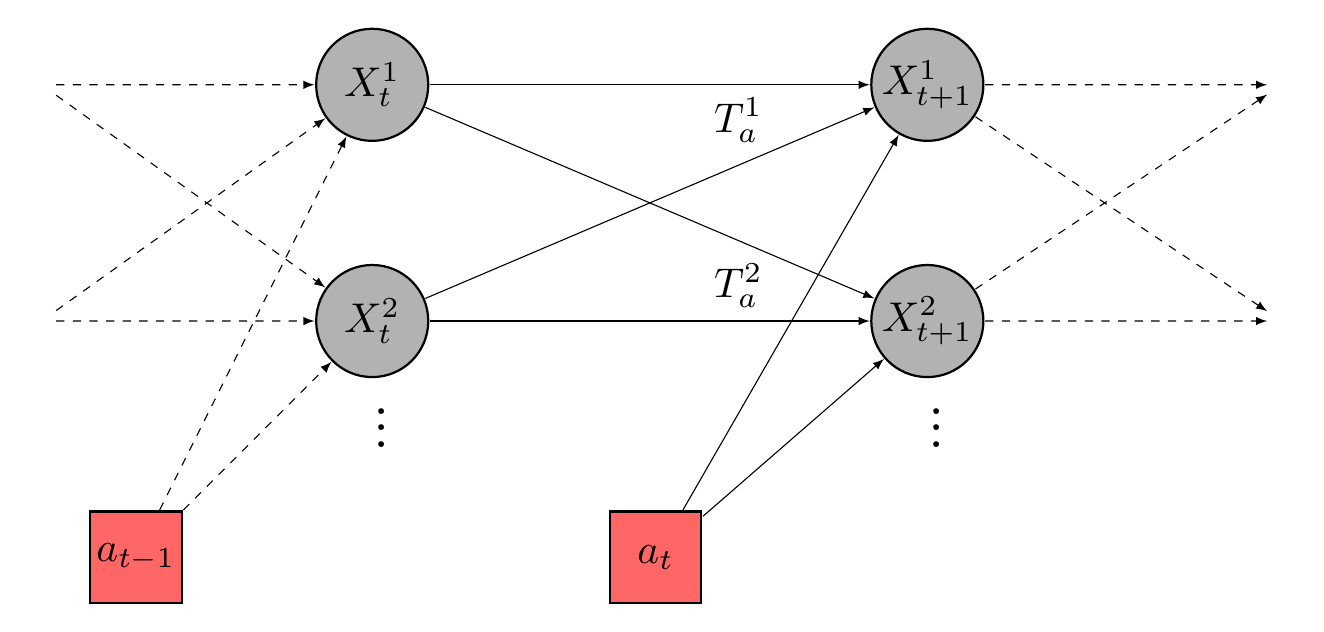
\begin{tikzpicture}[scale=1.5,transform shape]
%% vertex shape and color
\tikzstyle{vertex}=[circle,fill=black!30,minimum size=27pt,inner sep=0pt,draw=black,thick]
\tikzstyle{avertex}=[rectangle,fill=red!60,minimum size=22pt,inner sep=0pt,draw=black,thick]
\tikzstyle{rvertex}=[fill=yellow!60,decision=3,inner sep=-1pt,minimum size=35pt,draw=black,thick]
\definecolor{darkgreen}{rgb}{0.3,0.8,0.5}
\tikzstyle{overtex}=[circle,fill=blue!50,minimum size=35pt,inner sep=0pt,draw=black,thick]
%TIME
%\node [font=\huge] (statet) at (4,0.2) {$t$};
%\node [font=\huge] (statetplus1) at (9.2,0.2) {$t+1$};
%%%%%%%%%%%%%%%%%%%%%%%%%%%%%%%%%%%%%%%%%%%%%%%%%%%%%%%%%%%%%%%%%%%%%%%%
%1
\node[vertex] (state1) at (3.3,3) {$X^1_t$};
\node[vertex] (state12) at (3.3,1) {$X^2_t$};
\node (state13) at (3.3,0.2) {\begin{Large} $\vdots$ \end{Large}};
%2
\node[vertex] (state2) at (8,3) {$X^1_{t+1}$};
\node[vertex] (state22) at (8,1) {$X^2_{t+1}$};
\node (state23) at (8,0.2) {\begin{Large} $\vdots$ \end{Large}};

%0
\node (state0) at (0.5,3) {};
\node (state02) at (0.5,1) {};
%3
\node (state3) at (11,3) {};
\node (state32) at (11,1) {};

%%%%%%%%%%%%%%%%%%%%%%%%%%%%%%%%%%%%%%%%%%%%%%%%%%%%%%%%%%%%%%%%%%%%%%%%
%action
\node[avertex] (action) at (5.7,-1) {$a_t$};
\node[avertex] (action0) at (1.3,-1) {$a_{t-1}$};

%%%%%%%%%%%%%%%%%%%%%%%%%%%%%%%%%%%%%%%%%%%%%%%%%%%%%%%%%%%%%%
%ARROWS

%SV
% arrows sv->sv
%1->2
\draw[->,>=latex] (state1) -- (state2);
\draw[->,>=latex] (state1) -- (state22);
\draw[->,>=latex] (state12) -- (state2);
\draw[->,>=latex] (state12) -- (state22);
%0->1
\draw[->,>=latex,dashed] (state0) -- (state1);
\draw[->,>=latex,dashed] (state0) -- (state12);
\draw[->,>=latex,dashed] (state02) -- (state1);
\draw[->,>=latex,dashed] (state02) -- (state12);
%2->3
\draw[->,>=latex,dashed] (state2) -- (state3);
\draw[->,>=latex,dashed] (state2) -- (state32);
\draw[->,>=latex,dashed] (state22) -- (state3);
\draw[->,>=latex,dashed] (state22) -- (state32);

%A
% a->s
%1
\draw[->,>=latex] (action) -- (state2);
\draw[->,>=latex] (action) -- (state22);
%0
\draw[->,>=latex,dashed] (action0) -- (state1);
\draw[->,>=latex,dashed] (action0) -- (state12);

%%%%%%%%%%%%%%%%%%%%%%%%%%%%%%%%%%%%%%%%%%%%%%%%%%%%%%%%%%%%%%
% TRANSITION FUNCTIONS
\node (T1) at (6.4,2.7) {$T^1_a$};
\node (T2) at (6.4,1.3) {$T^2_a$};
\end{tikzpicture}
\caption[Dynamic Bayesian Network of a factored ($\pi$-)MDP]
{Dynamic Bayesian Network of a factored ($\pi$-)MDP:
in the possibilistic (resp. probabilistic) 
framework $T^i_a$ is the transition possibility (resp. probability) 
distribution of next variable $X^i_{t+1}$ conditional to
the selected action $a \in \mathcal{A}$
and its parents $parents(X^i_{t+1}) \subseteq \set{X^1_t,\ldots,X^n_t}$
(\textit{i.e.} $parents(X^i_{t+1})$ is a subset of the current state variables)
where $n\geqslant1$ is the number of variables describing the state space.
}
\label{fig_piMDPFact}
\end{figure}
In DBN semantics 
$parents(X^i_{t+1})$ is the set of state variables on which the next state variable $X^i_{t+1}$ ``depends'',
\textit{i.e.} a variable $Y$, represented by a node in the DBN, 
is in $parents(X^i_{t+1})$ if and only if there is an arrow from $Y$ to $X^j_{t+1}$.
We assume that $parents(X^i_{t+1}) \subseteq \set{X^1_t,\ldots,X^n_t}$,
\textit{i.e.} parents of the next state variable $X^i_{t+1}$
are a part of the current state variables $\set{X^1_t,\ldots,X^n_t}$:
there cannot be any arrow between state variables of the same time step.
Methods are discussed in the literature to circumvent this restrictive assumption
\cite{DBLP:conf/uai/Boutilier97}. 

As recalled in Section \ref{section_MarkovChains}, 
in probabilistic settings, 
the absence of an arrow in a Bayesian Network
represents an independence assumption. 
Let us consider a set of variables
$\set{Y_1, \ldots, Y_p}$, with $p>1$, 
and such that 
$\forall i \in \set{1,\ldots,p}$, $Y_i \in \mathcal{Y}_i$ 
where $\mathcal{Y}_i$ is a finite set.
For each $i \in \set{1,\ldots,p}$, 
the set of the parents of variables $Y_i$
can be denoted by 
$parents(Y_i) = \set{ Y_{pa_i(1)}, \ldots, Y_{pa_i(p_i)} } \subseteq \set{ Y_1,\ldots,Y_p }$,
where $pa_i: \set{1,\ldots,p_i} \rightarrow \set{1,\ldots,p}$ is an increasing function.
(note that $p_i \leqslant p$).
Let us recall that $children(Y_i)$ is the set of all the variables $Y_j \in \set{ Y_1,\ldots,Y_p }$ 
such that there is an arrow from $Y_i$ to $Y_j$.
The set $descend(Y_i)$ is the set of the descendants of variable $Y_i$:
$descend(Y_i)$ is defined as the smalest set containing $children(Y_i)$,
and such that $\forall Y_j \in descend(Y_i)$, $children(Y_j) \subset descend(Y_i)$.
The set of non-descendants 
$nondescend(Y_i) = \Big\{ Y_j \in \set{ Y_1,\ldots,Y_p } \ \Big\vert \ Y_j \notin \set{Y_i} \cup descend(Y_i) \cup parents(Y_i)  \Big\}$
can be also denoted by $\set{ Y_{nd_i(1)}, \ldots, Y_{nd_i(d_i)} } \subset \set{ Y_1,\ldots,Y_p }$
where $nd_i: \set{1,\ldots,d_i} \rightarrow \set{1,\ldots,n}$ is an increasing function (and $d_i \leqslant p$).
Hence, a DBN makes the assumption that
$Y_i$ is independent from its non-descendants conditional on its parents:
$Y_i \ \ \perp\!\!\!\perp \ \ nondescend(Y_i) \ \ \vert \ \ parents(Y_i)$.
In the probabilistic case, it can be written
$\forall (y_1,\ldots,y_p) \in \mathcal{Y}_1 \times \ldots \times \mathcal{Y}_p$,
$\forall i \in \set{1,\ldots p}$,
\[\mathbb{P} \paren{ Y_i=y_i \ \Big\vert \ Y_{pa_i(1)}=y_{pa_i(1)},\ldots, Y_{pa_i(p_i)}=y_{pa_i(p_i)}, Y_{nd_i(1)} = y_{nd_i(1)}, \ldots, Y_{nd_i(d_i)} = y_{nd_i(d_i)} }  \]
\begin{equation}
\label{DBNindep_prob} 
= \mathbb{P} \paren{ Y_i=y_i \ \Big\vert \ Y_{pa_i(1)}=y_{pa_i(1)},\ldots, Y_{pa_i(p_i)}=y_{pa_i(p_i)} }.
\end{equation}
This equation holds with a subset of the non-descendants $N \subset nondescend(Y_i)$: 
it suffices to consider the probability distribution 
over the set $nondescend(Y_i)\setminus N$, 
and compute the mean of each parts of the equation with respect to it.
The upper part is the probability distribution conditional on the parents of $Y_i$ and on $C$,
and the lower part remains the same.

Using this formula, if we consider the state variables $(X^i_t)_{t \in \set{0,\ldots,H}}^{i \in \set{1,\ldots,n}}$
and actions $(a_t)_{t=0}^{H-1}$
of a factored MDP, 
denoting by $X_t$ the variables $(X^i_t)_{i=1}^n$,
we get from the DBN of Figure \ref{fig_piMDPFact} that
$\forall t \in \set{ 0,\ldots, H-1}$, $\forall (x_0,\ldots,x_{t+1}) \in \set{ \top, \bot }^{t+2}$, $\forall (a_0,\ldots,a_t) \in \mathcal{A}^{t+1}$,
\[ \mathbb{P} \paren{ X_{t+1}=x_{t+1} \sachant X_0=x_0, \ldots, X_t=x_t, a_0,\ldots,a_{t-1} } = \mathbb{P} \paren{ X_{t+1}=x_{t+1} \sachant X_t=x_t, a_t }, \]
which is nothing more than the Markov property,
justifying the definition of the transition probability distributions $\textbf{p}(x' \vert x, a)$,
$\forall (x,x') \in \set{ \top, \bot }^{2n}$ and $\forall a \in \mathcal{A}$.

Section \ref{qualitative_indep} details that Qualitative Possibility Theory 
admits more than one independence definition:
for instance, the non-interactivity independence (NI-independence, see Definition \ref{def_NIindep}) 
and the causal or min-based independence (M-independence, see Definition \ref{def_mbindep})
are two useful independence definitions for this chapter.
If a DBN models M-dependences (causal dependences) 
between variables, 
then Equation \ref{DBNindep_prob} holds 
replacing the probability measure $\mathbb{P}$ 
by the possibility measure $\Pi$:
\[\Pi \paren{ Y_i=y_i \ \Big\vert \ Y_{pa_i(1)}=y_{pa_i(1)},\ldots, Y_{pa_i(p_i)}=y_{pa_i(p_i)}, Y_{nd_i(1)} = y_{nd_i(1)}, \ldots, Y_{nd_i(d_i)} = y_{nd_i(d_i)} }  \]
\begin{equation}
\label{DBN_M_indep}
= \Pi \paren{ Y_i=y_i \ \Big\vert \ Y_{pa_i(1)}=y_{pa_i(1)},\ldots, Y_{pa_i(p_i)}=y_{pa_i(p_i)} },
\end{equation}
which also holds considering only a subset of the descendants.
The possibilistic Markov property is also deduced from 
the DBN of Figure \ref{fig_piMDPFact} the same result for $\pi$-MDPs:
$\forall t \in \set{ 0,\ldots, H-1}$, $\forall (x_0,\ldots,x_{t+1}) \in \set{ \top, \bot }^{t+2}$, $\forall (a_0,\ldots,a_t) \in \mathcal{A}^{t+1}$,
\[ \Pi \paren{ X_{t+1}=x_{t+1} \sachant X_0=x_0, \ldots, X_t=x_t, a_0,\ldots,a_{t-1} } = \Pi \paren{ X_{t+1}=x_{t+1} \sachant X_t=x_t, a_t }, \]
which has been already defined in Section \ref{subsection_piMDPs}, see Equation \ref{equation_possmarkov}.

Consider again variables $(Y)_{i=1}^n$.
Let $A$ and $B$ be two disjoint subsets
of $\set{1,\ldots,n}$. 
In order to simplify notations,
if the probability 
$\mathbb{P} \paren{ (Y_i=y_i)_{i \in A} \sachant (Y_j=y_j)_{j \in B}  }$
is considered $\forall (y_i)_{i \in A} \in \bigtimes_{i \in A} \mathcal{Y}_i$
and $\forall(y_i)_{i \in B} \in \bigtimes_{i \in B} \mathcal{Y}_i$,
the probability can be denoted by 
$\mathbb{P} \paren{ (Y_i)_{i \in A} \sachant (Y_j)_{j \in B} }$.
For instance, Equation \ref{DBNindep_prob} can be rewritten
\[ \mathbb{P} \paren{ Y_i \ \Big\vert \ parents(Y_i), nondescend(Y_i) } = \mathbb{P} \paren{ Y_i \ \Big\vert \ parents(Y_i) }. \]

Let $(i_k)_{k=1}^s$ be an increasing sequence of indices  with $s \leqslant p$,
defining the set of variables $\set{Y_{i_1}, \ldots, Y_{i_k}}$.
The parents of variables $\set{Y_{i_1}, \ldots, Y_{i_k}}$ are
\[ parents \Big( (Y_{i_k})_{k=1}^s \Big) := \displaystyle \bigcup_{k=1}^s parents(Y_{i_k}). \]
Suppose that the set of variables $\set{Y_{i_1}, \ldots, Y_{i_k}}$
is such that %$\forall k \in \set{1,\ldots,s}$, 
$parents \Big( (Y_{i_k})_{k=1}^s \Big) \cap \set{Y_{i_1},\ldots,Y_{i_k}} = \emptyset$,
\textit{i.e.} the parents of variables $\set{Y_{i_1},\ldots,Y_{i_k}}$ 
are not in $\set{Y_{i_1},\ldots,Y_{i_k}}$.
Then, using the equation (\ref{DBNindep_prob}),  
we can write \\
$\mathbb{P} \paren{ (Y_{i_k})_{k=1}^s \ \bigg\vert \  parents \Big( (Y_{i_k})_{k=1}^s \Big)  }$
\begin{align*}
\hspace{3cm} &= \mathbb{P} \paren{ Y_{i_1} \ \bigg\vert \  parents \Big( (Y_{i_k})_{k=1}^s \Big)  } \cdot \mathbb{P} \paren{ Y_{i_2} \ \bigg\vert \  Y_{i_1}, parents \Big( (Y_{i_k})_{k=1}^s \Big)  } \cdot \\
&\hspace{2cm} \ldots \cdot \mathbb{P} \paren{ Y_{i_s} \ \bigg\vert \ Y_{i_1}, \ldots, Y_{i_{s-1}},  parents \Big( (Y_{i_k})_{k=1}^s \Big)  }  \\
&= \prod_{k=1}^s \mathbb{P} \Big( Y_{i_k} \ \Big\vert \ parents(Y_{i_k})   \Big).
\end{align*}
As already noted, the variables of the factored MDP model depicted by Figure \ref{fig_piMDPFact},
are such that $\forall t \geqslant 0$, $\forall i \in \set{1,\ldots,n}$, 
$parents(X^i_{t+1}) \subseteq \set{ X^1_t,\ldots,X^n_t }$:
thus, using the previous general equation (with variables $(Y_i)_{i=1}^p$), 
%$\forall (x^1_t,\ldots,x^n_t,x^1_{t+1},\ldots,x^n_{t+1})=(x_t,x_{t+1}) \in \set{ \top, \bot}^{2n}$,
\begin{align*}
\mathbb{P} \paren{ X_{t+1} \sachant X_t, a_t } &= \mathbb{P} \paren{ X^1_{t+1}, \ldots, X^n_{t+1} \sachant X_t, a_t }\\
&= \prod_{i=1}^{n} \mathbb{P} \Big( X^i_{t+1} \ \Big\vert parents(X^i_{t+1}), a_t \Big). 
\end{align*}
It shows that the transition probability distributions $\textbf{p} \paren{x' \sachant x,a}$ 
can be computed from the simpler distributions 
$\mathbb{P} \paren{ X^i_{t+1} \sachant parents(X^i_{t+1}), a_t  }$, $\forall i \in \set{1,\ldots,n}$.
These transition distributions are denoted by $\textbf{p} \paren{ X_i' \sachant parents(X_i'), a }$,
and by $T^i_a$ in Figure \ref{fig_piMDPFact}.
 
If we consider that the DBN involving variables $(Y_i)_{i=1}^k$ 
represents the M-dependences, 
Equation \ref{DBN_M_indep} holds, 
and using the definition 
of the qualitative possibilistic conditioning 
(Definition \ref{def_cond}),
we can also write \\
$\Pi \paren{ (Y_{i_k})_{k=1}^s \ \bigg\vert \  parents \Big( (Y_{i_k})_{k=1}^s \Big)  }$
\begin{align*}
\hspace{3cm} &= \min \Bigg\{ \Pi \paren{ Y_{i_1} \ \bigg\vert \  parents \Big( (Y_{i_k})_{k=1}^s \Big)  }, \Pi \paren{ Y_{i_2} \ \bigg\vert \  Y_{i_1}, parents \Big( (Y_{i_k})_{k=1}^s \Big)  }, \\
&\hspace{2cm} \ldots, \Pi \paren{ Y_{i_s} \ \bigg\vert \ Y_{i_1}, \ldots, Y_{i_{s-1}},  parents \Big( (Y_{i_k})_{k=1}^s \Big)  } \Bigg\}  \\
&= \min_{k=1}^s \Pi \Big( Y_{i_k} \ \Big\vert \ parents(Y_{i_k})   \Big),
\end{align*}
under the same assumption: $parents \Big( (Y_{i_k})_{k=1}^s \Big) \cap \set{Y_{i_1},\ldots,Y_{i_k}} = \emptyset$. 
Thus, as we consider that 
the DBN in Figure \ref{fig_piMDPFact}
represents the M-dependences,
\begin{align*}
\Pi \paren{ X_{t+1} \sachant X_t, a_t } &= \Pi \paren{ X^1_{t+1}, \ldots, X^n_{t+1} \sachant X_t, a_t }\\
&= \min_{i=1}^{n} \Pi \Big( X^i_{t+1} \ \Big\vert parents(X^i_{t+1}), a_t \Big). 
\end{align*}
The transition possibility distributions $\pi \paren{x' \sachant x,a}$ 
can be computed from the simpler distributions 
$\Pi \paren{ X^i_{t+1} \sachant parents(X^i_{t+1}), a_t  }$, $\forall i \in \set{1,\ldots,n}$,
denoted by $\pi \paren{ X^i_{t+1} \sachant parents(X^i_{t+1}), a }$,
and by $T^i_a$ in Figure \ref{fig_piMDPFact}.

With the $\pi$-MOMDP notations, assumptions of the Bayesian Network
in Figure \ref{fig_piMDPFact}
allows us to compute the joint possibility transition as 
$\pi \paren{s_v',\beta_h' \sachant s_v,\beta_h,a} = \pi \paren{ X' \sachant X,a } = \min_{i=1}^{n} \pi \paren{ X_i' \sachant parents(X_i'),a}$,
where, given a time step $t$, 
primed variables are variables concerning the time step $t+1$
(next variables), and non-primed variables are current variables 
(at time step $t$): for instance, 
$X_i'$ is the notation for $X^i_{t+1}$,
and $X_i$ the one for $X_t^i$.
Thus, a factored $\pi$-MOMDP can be defined 
with transition functions $T^i_a= \pi \paren{X_i' \sachant parents(X_i'),a }$ 
for each action $a$ and variable $X_i'$
(if transitions are assumed stationary).
% such that $T^{a,i}(parents(X_i'),a,X_i') = \pi \paren{\mathbb{X}_i' \sachant parents(\mathbb{X}_i'),a }$.

Each transition function can be compactly encoded in an Algebraic Decision
Diagram (ADD) \cite{Bahar:1997:ADD}. 
An ADD, as illustrated in Figure \ref{fig_ADDtransition}, 
is a directed acyclic graph which compactly represents a
real-valued function of binary variables, whose identical sub-graphs are
merged and zero-valued leaves are not memorized. 
The following notations are used to make it 
explicit that we are working with symbolic functions encoded as ADDs:
\begin{itemize}
\item $\ovalbox{$\min$} \set{f,g}$ where $f$ and $g$ are 2 ADDs;
\item $\ovalbox{$\max$}_{X_i} f$ = $\ovalbox{$\max$} \set{ f^{X_i=0},f^{X_i=1} }$, 
\end{itemize}
which can be easily computed because ADDs are constructed on the basis of the 
Shannon expansion: $f = \overline{X_i} \cdot f^{X_i=0} + X_i \cdot f^{X_i=1}$ 
where $f^{X_i=1}$ and $f^{X_i=0}$ are sub-ADDs representing the positive and 
negative Shannon cofactors (see Fig. \ref{fig_ADDtransition}). 

The optimistic possibilistic update of dynamic programming, 
\emph{i.e.} line \ref{VIupdate_OptAlgo} 
of the Value Iteration Algorithm \ref{algorithmIVPIMDP} 
in the previous chapter,
(or line \ref{piMOMDP_VIupdate} of the VI Algorithm \ref{algorithmpiMOMDP} for $\pi$-MOMDPs)
%equation of Line \ref{alg_piMDP_DP} of Algorithm \ref{algorithmIVPIMDP}
can be rewritten in a symbolic form, so that states are
now globally updated at once instead of individually: 
denoting by $X=(X_1,\ldots,X_n)$ the current variable
and $X'=(X_1',\ldots,X_n')$ the next one,
the possibilistic Q-value of an action $a \in \mathcal{A}$
%in a state $x \in \mathcal{X}$,
is $\overline{q^a} = \overline{q^a}(X)= \ovalbox{$\max$}_{X'} \ovalbox{$\min$} \set{ \pi \paren{ X' \sachant X,a }, \overline{U^*}(X') }$.
The computation of this ADD ($\overline{q^a}$) can be decomposed into independent computations 
thanks to the following proposition:
\begin{Property}[Possibilistic regression of the Value Function]
\label{propositionRegression}
Consider the current value function
 $\overline{U^*}: \set{\top,\bot}^n \rightarrow \mathcal{L}$. 
For a given action $a \in \mathcal{A}$, let us define:
\begin{itemize}
\item $\overline{q^a_0} = \overline{U^*}(X'_1,\cdots,X'_n)$, 
\item $\overline{q^a_i} = \max_{X'_i \in \set{\top,\bot}} \min \Big\{ \pi \paren{X_i' \sachant parents(X_i'),a} , \overline{q^a_{i-1}} \Big\}$.
\end{itemize}
Then, the possibilistic Q-value of action $a$ is: $\overline{q^a} = \overline{q^a_n}$,
which depends on variables $X_1,\ldots,X_n$,
and the next value function is $\overline{U^*}(X_1,\ldots,X_n) = \max_{a \in \mathcal{A}} \overline{q^a_n}(X_1,\ldots,X_n)$.
\end{Property}
The proof is given in Annex \ref{propositionRegression_RETURN}.
Note that the same trick can be used to compute 
pessimistic value functions,
using the equation (\ref{equationmaxmin4}) of Property \ref{property_minmax}: 
\begin{itemize}
\item $\underline{q^a_0} = \underline{U^*}(X'_1,\cdots,X'_n)$, 
\item $\underline{q^a_i} = \min_{X'_i \in \set{\top,\bot}} \max \Big\{ 1 - \pi \paren{X_i' \sachant parents(X_i'),a} , \underline{q^a_{i-1}} \Big\}$,
\end{itemize}
and next value function is $\underline{U^*}(X_1,\ldots,X_n) = \max_{a \in \mathcal{A}} \underline{q^a_n}(X_1,\ldots,X_n)$.

The Q-value of action $a$, represented as an ADD, can be then 
iteratively regressed over successive post-action state variables $X'_i ,
1 \leqslant i \leqslant n$. 
\begin{figure}
\centering
\begin{subfigure}[b]{0.35\linewidth}
\flushleft
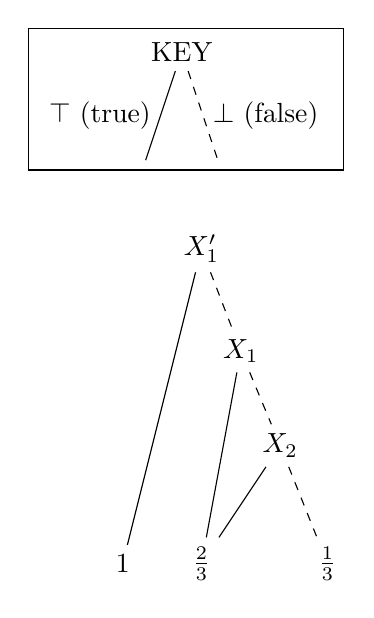
\begin{tikzpicture}
\draw (-1.2,5.5) rectangle (2.8,7.3);
\draw (0.75,7) node (key) {KEY};
\draw (0.25,5.5) node (Lt) {};
\draw (1.25,5.5) node (Lf) {};
\draw (key) -- (Lt) node [left,midway] {$\top$ (true)};
\draw [dashed] (key) -- (Lf) node [right,midway] {$\bot$ (false)};

\draw (1,4.5) node (Xp1) {$X_1'$};
\draw (0,0.5) node (L3) {$1$};
\draw (1.5,3.2) node (X11) {$X_1$};
\draw (2,2) node (X2) {$X_2$};
\draw (1,0.5) node (L1) {$\frac{2}{3}$};
\draw (2.6,0.5) node (L2) {$\frac{1}{3}$};
\draw [dashed] (Xp1) -- (X11);
\draw (X11) -- (L1);
\draw [dashed] (X11) -- (X2);
\draw (X2) -- (L1);
\draw [dashed] (X2) -- (L2);
\draw (Xp1) -- (L3);
\end{tikzpicture}
\caption{ADD encoding $T^a_1$ of Fig. \ref{fig_piMDPFact}\\\\}
\label{fig_ADDtransition}
\end{subfigure}
\qquad
\begin{subfigure}[b]{0.58\linewidth}
\flushright
\begin{tikzpicture}

\draw (-2,3) node {\ovalbox{$\min$} $\Bigg\{$};

\draw (0,4.5) node (Xp1) {$X'_1$};
\draw (1,3) node (Xp2) {$X'_2$};
\draw (-1,1.5) node (Lp1) {$\frac{1}{3}$};
\draw (0.5,1.5) node (Lp2) {$\frac{2}{3}$};
\draw (2,1.5) node (Lp3) {$0$};
\draw (Xp1) -- (Lp1);
\draw [dashed] (Xp1) -- (Xp2);
\draw (Xp2) -- (Lp2);
\draw [dashed] (Xp2) -- (Lp3);

\draw (2.2,3) node {,};

\draw (4,4.5) node (Xp1) {$X_1'$};
\draw (3,1.5) node (L3) {$1$};
\draw  (Xp1) -- (L3);
\draw (4.6,3.5) node (X11) {$X_1$};
\draw (5.2,2.5) node (X2) {$X_2$};
\draw (4,1.5) node (L1) {$\frac{2}{3}$};
\draw (5.7,1.5) node (L2) {$\frac{1}{3}$};
\draw (X11) -- (L1);
\draw [dashed] (X11) -- (X2);
\draw (X2) -- (L1);
\draw [dashed] (X2) -- (L2);
\draw [dashed] (Xp1) -- (X11);


\draw (6.3,3	) node {$\Bigg\}$};



\draw (-2,-1.3) node {=};
%\draw (-0.5,-1.3) node {=};


\draw (-0.7,0.5) node (rXp1) {$X'_1$};
\draw (0.5,-0.2) node (rXp2) {$X'_2$};
\draw (-0.2,-1.2) node (rX1) {$X_1$};
\draw (0.7,-2) node (rX2) {$X_2$};
\draw (-0.5,-3.2) node (rL1) {$\frac{2}{3}$};
\draw (1.3,-3.2) node (rL2) {$\frac{1}{3}$};
\draw (-1.5,-3.2) node (rL3) {$\frac{1}{3}$};
\draw (2,-3.2) node (rL4) {$0$};

\draw [dashed] (rXp1) -- (rXp2);
\draw  (rXp2) -- (rX1);
\draw [dashed] (rXp2) -- (rL4);
%\draw (rXp2) -- (rX1);
%\draw [dashed] (rXp2) -- (rL3);
\draw (rXp1) -- (rL3);
\draw (rX1) -- (rL1);
\draw [dashed] (rX1) -- (rX2);
\draw (rX2) -- (rL1);
\draw [dashed] (rX2) -- (rL2);

%\draw (0.3,-2) node (dL1) {$\frac{1}{3}$};
%\draw (rXp1) -- (rL1);

\draw (2.5,-1.3) node {$\xrightarrow[\text{\ovalbox{$\max$}}_{X'_1}]{}$};

%\draw (4.5,-2) node (rrXp2) {$\mathbb{X}'_2$};
\draw (4.8,0.5) node (rrpX2) {$X_2'$};
\draw (4,-0.5) node (rrX1) {$X_1$};
\draw (4.5,-1.7) node (rrX2) {$X_2$};
\draw (3.5,-3.2) node (rrL1) {$\frac{2}{3}$};
\draw (5.7,-3.2) node (rrL2) {$\frac{1}{3}$};
\draw (rrpX2) -- (rrX1);
\draw (rrX1) -- (rrL1);
%\draw (rrXp2) -- (rrX1);
\draw [dashed] (rrX1) -- (rrX2);
\draw (rrX2) -- (rrL1);
\draw [dashed] (rrX2) -- (rrL2);
\draw [dashed] (rrpX2) -- (rrL2);



%\draw (2,-1) node (rXp1) {$X'_1$};
%\draw (2.5,-2) node (rXp2) {$X'_2$};
%\draw (1.7,-3) node (rX1) {$X_1$};
%\draw (2,-4) node (rX2) {$X_2$};
%\draw (1,-5) node (rL1) {$\frac{2}{3}$};
%\draw (2.5,-5) node (rL2) {$\frac{1}{3}$};
%\draw (3,-3) node (rL3) {$0$};

%\draw [dashed] (rXp1) -- (rXp2);
%\draw (rXp2) -- (rX1);
%\draw [dashed] (rXp2) -- (rL3);
%\draw (rX1) -- (rL1);
%\draw [dashed] (rX1) -- (rX2);
%\draw (rX2) -- (rL1);
%\draw [dashed] (rX2) -- (rL2);

%\draw (1,-2) node (gXp2) {$X'_2$};
%\draw (0.5,-3) node (dL1) {$\frac{1}{3}$};
%\draw [dashed] (gXp2) -- (rX1);
%\draw (gXp2) -- (dL1);
%\draw (rXp1) -- (gXp2);
%\draw (3.5,-3.5) node {$\xrightarrow[\text{\ovalbox{$\max$}}_{X'_1,X'_2}]{}$};%

%\draw (5,-2) node (rrX1) {$X_1$};
%\draw (5.5,-3) node (rrX2) {$X_2$};
%\draw (4.5,-4) node (rrL1) {$\frac{2}{3}$};
%\draw (6,-4) node (rrL2) {$\frac{1}{3}$};
%\draw (rrX1) -- (rrL1);
%\draw [dashed] (rrX1) -- (rrX2);
%\draw (rrX2) -- (rrL1);
%\draw [dashed] (rrX2) -- (rrL2);
\end{tikzpicture}
\caption{Symbolic regression of the current Q-value ADD combined with the transition ADD of Figure \ref{fig_ADDtransition}\\}
\label{fig_ADDregression}
\end{subfigure}
\caption{Algebraic Decision Diagrams for PPUDD}
\label{fig_ADD}
\end{figure}	
Figure \ref{fig_ADDregression} illustrates the possibilistic regression of the
Q-value of an action for the first state variable $X_1$ and leads to the intuition that ADDs should be far 
smaller in practice under possibilistic settings, since their leaves lie in $\mathcal{L}$ instead
of $\mathbb{R}$, thus yielding more sub-graph simplifications.

% Contrary to factored
%\emph{probabilistic} MDPs, for which additions and multiplications involved in
%the computation of Q-values create new values (i.e. ADD leaves) most of the
%time, factored $\pi$-MOMDPs' $\min$ and $\max$ operations do not create new values
%from the input ADDs. More concretely, ADDs with probabilistic operations can have up to
%$2^n$ leaves (i.e. as many values as the number of states), whereas ADDs with
%possibilistic operations can have up to $\#\mathcal{L} \ll 2^n$ leaves. It means that
%ADDs should be far smaller in practice under possibilistic settings, which was a
%motivation for this paper and is experimentally checked in a forthcoming
%section.

\begin{algorithm} \caption{PPUDD (infinite horizon resolution)} \label{PPUDD} 
 $\overline{U^*} \gets 0$ ;
 $\overline{U^c} \gets \Psi$ ;
 $\overline{\delta} \gets \widehat{a}$ \;

\While {$\overline{U^*} \neq \overline{U^c}$ \label{while_PPUDD} }{
 $\overline{U^*} \gets \overline{U^c}$ \;
 \For {$a \in \mathcal{A}$ \label{ppuddBeginQ}}{
	$\overline{q^a}  \gets $ swap each $X_i$ variable in $\overline{U^*}$ with $X_i'$ \label{ppuddSwap} \;
	\For {$1 \leqslant i \leqslant n$}{
	 $\overline{q^a} \gets \ovalbox{$\min$} \ \bigg\{ \overline{q^a} , \pi \Big( X_i' \ \Big\vert parents(X_i'),a \Big) \bigg\}$ \;
	 $\overline{q^a} \gets \ovalbox{$\max$}_{X_i'} \overline{q^a}$ \;
	}
	$\overline{U^c} \gets \ovalbox{$\max$} \set{\overline{q^a},\overline{U^c}  } $ \label{ppuddEndQ} \;
	update $\overline{\delta}$ to $a$ where $\overline{q^a}=\overline{U^c}$ and $\overline{U^c} > \overline{U^*}$ \;
}
}
\Return $\overline{U^*}$, $\overline{\delta^*}$ \;
\end{algorithm}

Algorithm \ref{PPUDD} is a symbolic version of the $\pi$-MOMDP Value Iteration Algorithm (Algorithm \ref{algorithmpiMOMDP} in the previous chapter),
which relies on the regression scheme defined in Proposition
\ref{propositionRegression}. Inspired by SPUDD \cite{Hoey99spudd:stochastic},
PPUDD means \emph{Possibilistic Planning Using Decision Diagrams}. As for SPUDD,
it needs to swap unprimed state variables to primed ones in the ADD encoding the
current value function before computing the Q-value of an action $a$ (see Line
\ref{ppuddSwap} of Algorithm \ref{PPUDD} and Figure \ref{fig_ADDregression}). This operation is required to
differentiate the next state represented by primed variables from the
current one when operating on ADDs. Lines \ref{ppuddBeginQ}-\ref{ppuddEndQ} apply
Proposition \ref{propositionRegression} and correspond to Line
\ref{VIupdate_OptAlgo} of Algorithm \ref{algorithmIVPIMDP}.

We mentioned at the beginning of this section 
that belief state space $\Pi^{\mathcal{S}_h}_{\mathcal{L}}$
could be described by $\lceil \log_2 K \rceil$ binary variables where $K=\#
\mathcal{L}^{\#\mathcal{S}_h} - (\# \mathcal{L}-1)^{\# \mathcal{S}_h}$. 
However, this $K$ can be
very large so we propose 
in the next section a method to exploit the
factorization of $\mathcal{S}_h$ and $\mathcal{O}_h$ 
in order to factorize $\Pi^{\mathcal{S}_h}_{\mathcal{L}}$
itself into small belief subvariables, which will decompose the possibilistic
transition ADD into an aggregation of smaller ADDs.
Note that PPUDD can solve $\pi$-MOMDPs even if this belief factorization is not 
feasible, but it will manipulate bigger ADDs.

Previous chapter highlight that 
a pre-treatment is required to translate
a $\pi$-MOMDP into a $\pi$-MDP whose state space is $\mathcal{X}$.
We can then reason on the state space accessible to the agent 
$\mathcal{X} = S_v \times \Pi^{\mathcal{S}_h}_{\mathcal{L}}$ and
solve the $\pi$-MOMDP as a $\pi$-MDP.
Next section links the structured properties of a $\pi$-MOMDP,
concerning dependencies of original variables (visible, hidden and observation ones), 
to the factorization of the treated problem \textit{i.e.} of the resulting $\pi$-MDP 
on $S_v \times \Pi^{\mathcal{S}_h}_{\mathcal{L}}$ (concerning dependencies of visible and belief variables).

Finally, we note that we could have used \emph{complete action diagrams} (CADs)
introduced in \cite{St-aubin00apricodd:approximate}, 
which directly encode the
transition matrix of each action as a single ADD.
On one hand, CADs are simpler
to manipulate than a set of transition ADDs for each state variable, and enable
to deal with correlated action effects. On the other hand,
they require to
operate bigger ADDs while preventing intermediate simplifications that are yet
offered by reasoning about separate state variables as we do (Lines
\ref{ppuddBeginQ}-\ref{ppuddEndQ} of Algorithm \ref{PPUDD}) or SPUDD does
\cite{Hoey99spudd:stochastic}.

%%%%%%%%%%%%%%%%%%%%%%%%%%%%%%%%%%%%%%%%%%%%%%%%%%%%%%%%%%%%
%%%%%%%%%%%%%%%%%%%%%%%%%%%%%%%%%%%%%%%%%%%%%%%%%%%%%%%%%%%%
%%%%%%%%%%%%%%%%%%%%%%%%%%%%%%%%%%%%%%%%%%%%%%%%%%%%%%%%%%%%
%%%%%%%%%%%%%%%%%%%%%%%%%%%%%%%%%%%%%%%%%%%%%%%%%%%%%%%%%%%%
%%%%%%%%%%%%%%%%%%%%%%%%%%%%%%%%%%%%%%%%%%%%%%%%%%%%%%%%%%%%
%%%%%%%%%%%%%%%%%%%%%%%%%%%%%%%%%%%%%%%%%%%%%%%%%%%%%%%%%%%%
%%%%%%%%%%%%%%%%%%%%%%%%%%%%%%%%%%%%%%%%%%%%%%%%%%%%%%%%%%%%
%%%%%%%%%%%%%%%%%%%%%%%%%%%%%%%%%%%%%%%%%%%%%%%%%%%%%%%%%%%%
\section{$\pi$-MOMDP belief factorization}
%\subsection{Possibilistic Bayesian Networks and Independences}
%\subsection{The $\pi$-MOMDP case}
Factorizing the belief variable requires three structural assumptions on the 
$\pi$-MOMDP's DBN, which are illustrated by the Rocksample benchmark 
\cite{Smith:2004:HSV:1036843.1036906}.
\subsection{Motivating example.}
\label{section_RS_motivatingEx}
A rover navigating in a $g \times g$ grid has to collect scientific samples from 
interesting (``good'') rocks among $R$ ones and then to reach the exit. It is 
fitted with a noisy long-range sensor that can be used to determine if a rock 
is ``good'' or not.
It knows the locations of the $R$ rocks $(x_i,y_i)_{i=1}^R$ 
but not which ones are actually of interest (called ``good'' rocks). 
However, sampling a rock is expensive: 
the rover is fitted with a noisy long-range sensor that can be used to determine 
if a rock is ``good'' or not (``bad''). 
When a rock is sampled, 
it becomes (or stays) ``bad'' (no more interesting). 
At the end of the mission, the rover has to reach the exit location at the right side of the grid:
\begin{itemize}
\item $\mathcal{S}_{v}$ consists of all the possible locations of the rover %$(x_r,y_r)$ 
in addition to the exit ($\# \mathcal{S}_v = g^2 +1$);
\item $\mathcal{S}_h$ consists of all the possible natures of the rocks:
$\mathcal{S}_h = \mathcal{S}^1_h \times \ldots \times \mathcal{S}^R_h$,
with $\forall 1 \leqslant i \leqslant R$, $\mathcal{S}^i_h=\set{ good,bad }$;
\item $\mathcal{A}$ contains the (deterministic) moves in the $4$ directions ($a_{north},a_{east},a_{south},a_{west}$)
, checking rock $i$, ($a_{check_i}$) 
$\forall 1 \leqslant i \leqslant R $, 
and sampling the current rock, ($a_{sample}$);
\item $\mathcal{O} = \set{ o_{good},o_{bad} }$ are the possible sensor's answers for the current rock. 
% $\mathcal{O}_{1} \times \ldots \times \mathcal{O}_{R}$ where $\forall 1 \leqslant i \leqslant R$, $\mathcal{O}_{i}=\set{ o_{good},o_{bad} }$ are observations concerning the $i^{th}$ rock. \\
\end{itemize}

%Without going into details of the model, the factorization of the observation
%set naturally yields to the structural assumption required for factored
%$\pi$-MOMDPs, since each observation variable is mapped to a hidden state
%variable. 
%Note that the observation set of this domain is best known in the
%literature in the simpler form $\mathcal{O}=\{o_{good},o_{bad}\}$, where the
%observation concerns the current rock, which is strictly equivalent to the
%previous factorization but does not highlight the structure of the problem. 
The rationale behind observation dynamics is the following: 
the more the rover is close to
the checked rock, the better it observes its nature. 
In the original
probabilistic model, 
the probability of a correct observation equals
$\frac{1}{2}\paren{ 1 + e^{-c \sqrt{(x_r-x_i)^2 + (y_r-y_i)^2} }} $ with $c>0$.
 a constant (the smaller is $c$, the more effective is the sensor). 
The rover gets the reward $+10$ (resp. $-10$) for each good (resp. bad) sampled rock, % $-10$ for each bad rock sampled,
and $+10$ when it reaches the exit. 

In the possibilistic model, the observation function is approximated using a
critical distance $d>0$ beyond which checking a rock is uninformative: $\pi
\paren{ o_i' \sachant s_i',a,s_v } = 1$ $ \forall o_i' \in \mathcal{O}_{i} $.
%If the
%rover is distant from the rock less than $d$, 
The possibility degree of
erroneous observation becomes zero if it stands at
the checked rock, and lowest non zero possibility degree otherwise. Finally, 
as possibilistic semantics does not allow sums of
rewards, an additional visible state variable $s^2_v \in
\set{ 1, \ldots, R }$ which counts the number of checked rocks is introduced. 
The qualitative dislike of sampling is modeled as $\Psi(s)=\frac{R+2-s_{v,2}}{R+2}$
if the location is terminal and zero otherwise. 
%Preference $\Psi(s)$ equals qualitative dislike of sampling $\frac{R+2-s_{v,2}}{R+2}$ 
%if all rocks are bad and location is terminal, zero otherwise.
The location of the rover is finally denoted by $s^1_v \in \mathcal{S}^1_v$ and the visible state is then
$s_v=(s^1_v,s^2_v) \in \mathcal{S}^1_v \times \mathcal{S}^2_v = \mathcal{S}_v$. 

Observations $\set{ o_{good},o_{bad} }$ for the current rock can be equivalently 
modeled as a Cartesian product of observations $\set{ o_{good_1},o_{bad_1} } \times \cdots \times \set{ o_{good_R},o_{bad_R} }$ 
for each rock. By using this equivalent modeling, state and observation spaces 
are both respectively factored as 
$\mathcal{S}^1_v \times \ldots \times \mathcal{S}^m_v \times \mathcal{S}^1_h \times \ldots \times \mathcal{S}^l_h $
 and $\mathcal{O} = \mathcal{O}^1 \times \ldots \times \mathcal{O}^l$, and we can now map each observation variable 
$O^j \in \mathcal{O}^j$ to its hidden state variable $S^j_h \in \mathcal{S}^j_h$. 
It allows us to reason 
about the DBN of Figure \ref{fig_piMOMDPFact}, 
which expresses three important assumptions 
that will help us factorize the belief state itself:
\begin{enumerate}
\item all state variables $S^1_v,S^2_v,\ldots,S^m_v,S^1_h,S^2_h,\ldots,S^l_h$ are post-action independent 
variables, and next visible variables does not depend on current hidden ones.
Thus, there is no arrow between two state variables at the same time step, as $S^2_{v,t}$ and $S^1_{h,t}$,
nor arrow from a current hidden variable to a next visible one, as $S^1_{h,t}$ and $S^1_{v,t+1}$;
\item a hidden variable does not depend on previous other hidden variables: the nature of a rock is 
independent from the previous nature of other rocks. 
For instance, there is no arrow from $S^1_{h,t}$ to $S^2_{h,t+1}$;
\item an observation variable is available for each hidden state variable,
and depends on it. 
It does not depend on other 
hidden state variables 
nor current visible ones, 
but on previous visible state variables and action:
for instance, there is no arrow between $S^1_{h,t+1}$ and $O^2_{t+1}$, 
nor between $S^1_{v,t+1}$ and $O^1_{t+1}$. 
\end{enumerate}
Each observation 
variable is indeed only related 
to the nature of the corresponding rock. 
The observation quality yet depends on the rover's location 
\emph{i.e.} a current visible state variable, 
not allowed by the DBN: 
fortunately, as moves are deterministic, 
we avoid this issue considering observations depend on previous location and action.


\begin{figure}[b!]\centering
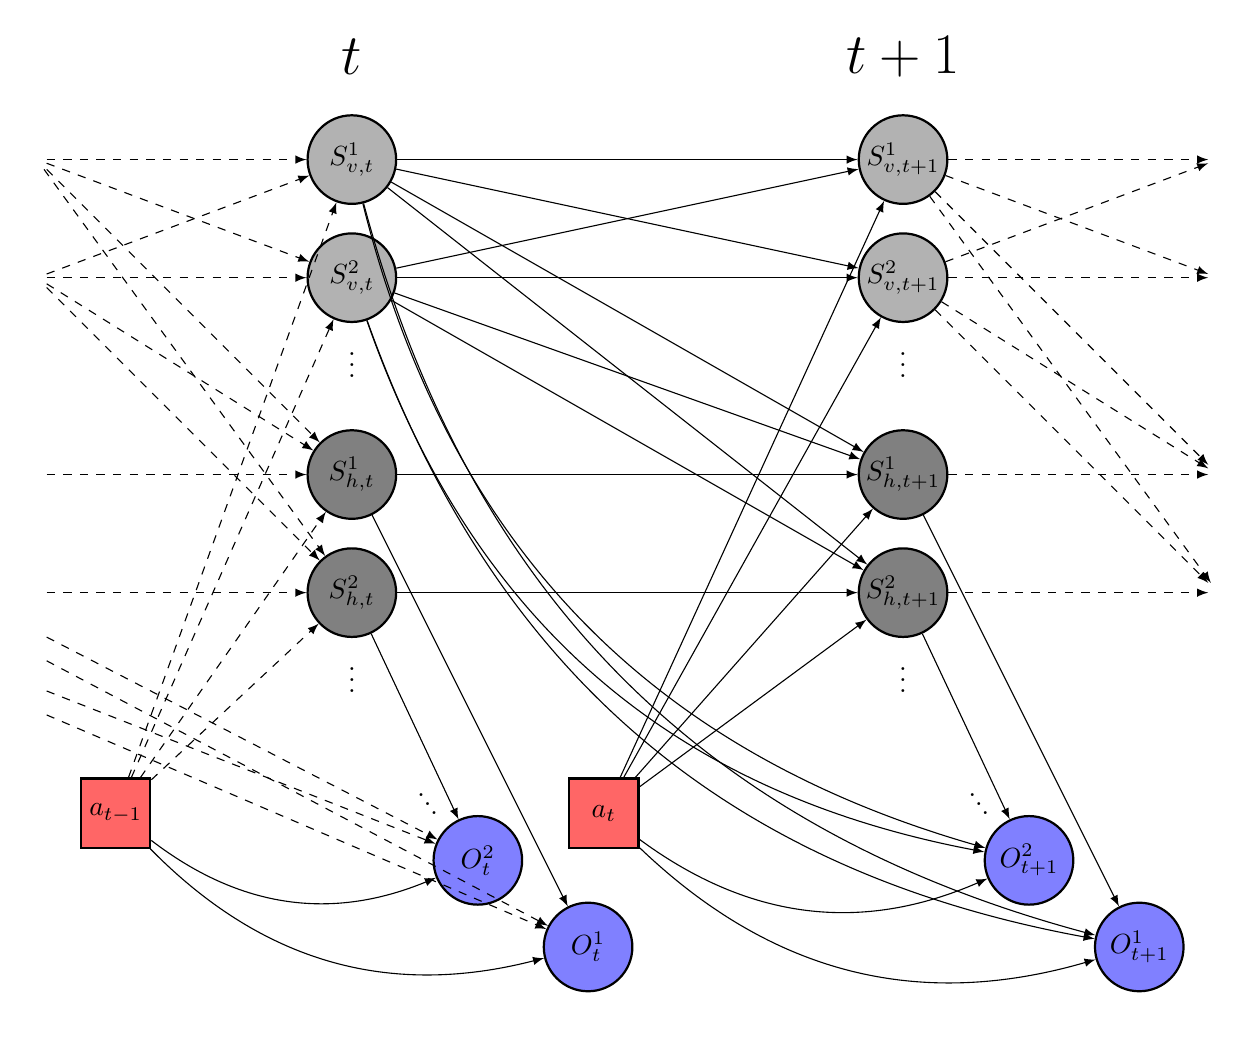
\begin{tikzpicture}
\tikzstyle{vertex}=[circle,fill=black!50,minimum size=32pt,inner sep=0pt,draw=black,thick]
\tikzstyle{vvertex}=[circle,fill=black!30,minimum size=32pt,inner sep=0pt,draw=black,thick]
\tikzstyle{avertex}=[rectangle,fill=red!60,minimum size=25pt,inner sep=0pt,draw=black,thick]
\tikzstyle{rvertex}=[fill=yellow!60,decision=3,inner sep=-1pt,minimum size=35pt,draw=black,thick]
\definecolor{darkgreen}{rgb}{0.3,0.8,0.5}
\tikzstyle{overtex}=[circle,fill=blue!50,minimum size=32pt,inner sep=0pt,draw=black,thick]


%TIME
\node [font=\huge] (statet) at (3,7.3) {$t$};
\node [font=\huge] (statetplus1) at (10,7.3) {$t+1$};
%%%%%%%%%%%%%%%%%%%%%%%%%%%%%%%%%%%%%%%%%%%%%%%%%%%%%%%%%%%%%%%%%%%%%%%%
%vstates
%1
\node[vvertex] (vstate1) at (3,6) {$S^1_{v,t}$};
\node[vvertex] (vstate12) at (3,4.5) {$S^2_{v,t}$};
\node (vstate13) at (3,3.5) {$\vdots$};
%2
\node[vvertex] (vstate2) at (10,6) {$S^1_{v,t+1}$};
\node[vvertex] (vstate22) at (10,4.5) {$S^2_{v,t+1}$};
\node (vstate23) at (10,3.5) {$\vdots$};

%0
\node (vstate0) at (-1,6) {};
\node (vstate02) at (-1,4.5) {};
%3
\node (vstate3) at (14,6) {};
\node (vstate32) at (14,4.5) {};


%%%%%%%%%%%%%%%%%%%%%%%%%%%%%%%%%%%%%%%%%%%%%%%%%%%%%%%%%%%%%%%%%%%%%%%%
%hstates
%1
\node[vertex] (hstate1) at (3,2) {$S^1_{h,t}$};
\node[vertex] (hstate12) at (3,0.5) {$S^2_{h,t}$};
\node (hstate13) at (3,-0.5) {$\vdots$};
%2
\node[vertex] (hstate2) at (10,2) {$S^1_{h,t+1}$};
\node[vertex] (hstate22) at (10,0.5) {$S^2_{h,t+1}$};
\node (hstate23) at (10,-0.5) {$\vdots$};
%0
\node (hstate0) at (-1,2) {};
\node (hstate02) at (-1,0.5) {};
%3
\node (hstate3) at (14,2) {};
\node (hstate32) at (14,0.5) {};



%%%%%%%%%%%%%%%%%%%%%%%%%%%%%%%%%%%%%%%%%%%%%%%%%%%%%%%%%%%%%%%%%%%%%%%%
%action
\node[avertex] (action) at (6.2,-2.3) {$a_t$};
\node[avertex] (action0) at (0,-2.3) {$a_{t-1}$};

%%%%%%%%%%%%%%%%%%%%%%%%%%%%%%%%%%%%%%%%%%%%%%%%%%%%%%%%%%%%%%%%%%%%%%%%
% observations
%1
\node[overtex] (hobserv1) at (6,-4) {$O^1_t$};
\node[overtex] (hobserv12) at (4.6,-2.9) {$O^2_t$};
\node (doto1) at (3.9,-2.1) [rotate=36] {$\vdots$};
%\node at (3.7,-3.3) {$\ldots$};
%2
\node[overtex] (hobserv2) at (13,-4) {$O^1_{t+1}$};
\node[overtex] (hobserv22) at (11.6,-2.9) {$O^2_{t+1}$};
\node (doto2) at (10.9,-2.1) [rotate=36] {$\vdots$};
%\node at (7.9,-3.4) {$\ldots$};


%%%%%%%%%%%%%%%%%%%%%%%%%%%%%%%%%%%%%%%%%%%%%%%%%%%%%%%%%%%%%%
%ARROWS

%SV
% arrows sv->sv
%1->2
\draw[->,>=latex] (vstate1) -- (vstate2);
\draw[->,>=latex] (vstate1) -- (vstate22);
\draw[->,>=latex] (vstate12) -- (vstate2);
\draw[->,>=latex] (vstate12) -- (vstate22);
%0->1
\draw[->,>=latex,dashed] (vstate0) -- (vstate1);
\draw[->,>=latex,dashed] (vstate0) -- (vstate12);
\draw[->,>=latex,dashed] (vstate02) -- (vstate1);
\draw[->,>=latex,dashed] (vstate02) -- (vstate12);
%2->3
\draw[->,>=latex,dashed] (vstate2) -- (vstate3);
\draw[->,>=latex,dashed] (vstate2) -- (vstate32);
\draw[->,>=latex,dashed] (vstate22) -- (vstate3);
\draw[->,>=latex,dashed] (vstate22) -- (vstate32);


% arrows sv->sh
%1->2
\draw[->,>=latex] (vstate1) -- (hstate2);
\draw[->,>=latex] (vstate1) -- (hstate22);
\draw[->,>=latex] (vstate12) -- (hstate2);
\draw[->,>=latex] (vstate12) -- (hstate22);
%0->1
\draw[->,>=latex,dashed] (vstate0) -- (hstate1);
\draw[->,>=latex,dashed] (vstate0) -- (hstate12);
\draw[->,>=latex,dashed] (vstate02) -- (hstate1);
\draw[->,>=latex,dashed] (vstate02) -- (hstate12);

%2->3
\draw[->,>=latex,dashed] (vstate2) -- (hstate3);
\draw[->,>=latex,dashed] (vstate2) -- (hstate32);
\draw[->,>=latex,dashed] (vstate22) -- (hstate3);
\draw[->,>=latex,dashed] (vstate22) -- (hstate32);


% arrows sv->oh

\draw[->,>=latex] (vstate1) to[bend right] (hobserv2);
\draw[->,>=latex] (vstate12) to[bend right] (hobserv2);
\draw[->,>=latex] (vstate1) to[bend right] (hobserv22);
\draw[->,>=latex] (vstate12) to[bend right] (hobserv22);


\node (fake0) at (-1,-1) {};
\node (fake1) at (-1,0) {};
\node (fake2) at (-1,-0.3) {};
\node (fake3) at (-1,-0.7) {};
\draw[->,>=latex,dashed] (fake0) to (hobserv1);
\draw[->,>=latex,dashed] (fake1) to (hobserv12);
\draw[->,>=latex,dashed] (fake2) to (hobserv1);
\draw[->,>=latex,dashed] (fake3) to (hobserv12);

%SH
% arrows sh->sh
%1->2
\draw[->,>=latex] (hstate1) -- (hstate2);
\draw[->,>=latex] (hstate12) -- (hstate22);
%0->1
\draw[->,>=latex,dashed] (hstate0) -- (hstate1);
\draw[->,>=latex,dashed] (hstate02) -- (hstate12);

%2->3
\draw[->,>=latex,dashed] (hstate2) -- (hstate3);
\draw[->,>=latex,dashed] (hstate22) -- (hstate32);

% arrows sh->oh
%1
\draw[->,>=latex] (hstate1) to (hobserv1);
\draw[->,>=latex] (hstate12) to (hobserv12);
%2
\draw[->,>=latex] (hstate2) to (hobserv2);
\draw[->,>=latex] (hstate22) to (hobserv22);

%A
% a->s
%1
\draw[->,>=latex] (action) -- (vstate2);
\draw[->,>=latex] (action) -- (vstate22);
\draw[->,>=latex] (action) -- (hstate2);
\draw[->,>=latex] (action) -- (hstate22);
%0
\draw[->,>=latex,dashed] (action0) -- (vstate1);
\draw[->,>=latex,dashed] (action0) -- (vstate12);
\draw[->,>=latex,dashed] (action0) -- (hstate1);
\draw[->,>=latex,dashed] (action0) -- (hstate12);

% a->oh
%1
\draw[->,>=latex] (action) to[bend right] (hobserv2);
\draw[->,>=latex] (action) to[bend right] (hobserv22);
%0
\draw[->,>=latex] (action0) to[bend right] (hobserv1);
\draw[->,>=latex] (action0) to[bend right] (hobserv12);

%\node (probao1) at (4,-2.2) [rotate=350] {$ \pi \paren{ o_{h,t} \sachant s_t, a_{t-1}}$};
%\node (probao2) at (11,-2.5) [rotate=350] {$ \pi \paren{ o_{h,t+1} \sachant s_{t+1}, a_{t}}$};
%\node (probas) at (8.9,0.5) [rotate=355] {$ \pi \paren{s_{t+1} \sachant s_t,a_{t}}$};

\end{tikzpicture}
\caption[DBN of a factored belief-independent $\pi$-MOMDP]{
DBN summing up independence assumptions of a $\pi$-MOMDP
leading to marginal beliefs and a $\pi$-MDP with 
a factored transition function \textit{i.e.} a factored belief $\pi$-MDP.
Parents of a visible state variable are the previous visible state variables.
Parents of a hidden state variable are the previous visible state variables 
and the corresponding previous hidden state variable. 
Finally,
parents of an observation variable are the previous visible state variables,
and the corresponding current hidden state variable.
}
\label{fig_piMOMDPFact}
\end{figure}

\subsection{Consequences of the factorization assumptions}
\label{section_factoAssumptions}
In this section, we formally demonstrate how the three previous independence assumptions can be
used to factorize $\Pi^{\mathcal{S}_h}_{\mathcal{L}}$ 
as the Cartesian product $\displaystyle \bigtimes_{j=1}^{l} \Pi^{\mathcal{S}^j_h}_{\mathcal{L}}$,
\textit{i.e.} represent the belief state $\beta_h$ about the hidden states $s_h \in \mathcal{S}_h$ 
with marginal belief states $\beta^j_h \in \Pi^{\mathcal{S}^j_h}_{\mathcal{L}}$
about hidden states $s^j \in \mathcal{S}^j_h$, $\forall j \in \set{1,\ldots,l}$.
% via the $\min$ aggregation:
%As in the probabilistic framework, the possibilistic belief at time step $t
%\geqslant 0$ is defined as the possibility distribution over variable $s_{h,t}$
%conditioned on history $h_t$: $\forall s_h \in \mathcal{S}_h$, $\beta_t(s_h) = \pi
%\paren{ s_h \sachant h_t }$. %if $s_{h,1}, \ldots,s_{h,l}$ are initially
% independent, then
% at each time
%step $t>0$ the belief over hidden states can be written $\beta_t =
% \min_{j=1}^{l} \beta_{t,j}$ with
%$\forall s_j \in \mathcal{S}_{h,j}$, $\beta_{t,j}(s_j) = \pi \paren{ s_j \sachant
% h_t }$ the belief over $\mathcal{S}_j$.

To this end, we will use \textit{d-Separation criterion} \cite{pearl88} 
in order to show some independence between variables from the DBN.
As explained in Section \ref{section_PPUDD}, 
a DBN can be drawn from independence relations.
Let us denote by $X \perp\!\!\!\perp Y \ \vert \ Z$
the assertion ``$X$ is independent from $Y$ conditional on $Z$'':
recall that for a given definition of the used independence relation,
e.g. probabilistic, non interactivity (NI), or minimum based (M, causal) independence,
the DBN is drawn such that for each node (variable) $X$,
$X \perp\!\!\!\perp nondescend(X) \ \vert \ parents(X)$.
If the used independence relation obey the \textit{semi-graphoids} axioms \cite{Pearl:1988:PRI:52121,DBLP:journals/corr/abs-1304-2379},
the graphical criterion called d-Separation 
can be used to identify some independences between variables of the DBN.

This criterion is for instance used in probabilistic settings in \cite{Witwicki13icaps}.
Recall that the M-independence is not symetric (see Section \ref{qualitative_indep}),
and thus does not obey the axioms of semi-graphoids.
However, the NI-independence leads to a semi-graphoids,
as proved in \cite{delafonk}.

Let us recall that M-independence implies NI-independence
(see Theorem \ref{theorem_NIequivalence} of Section \ref{qualitative_indep}).
The DBN of Figure \ref{fig_piMOMDPFact}
represents M-independences between variables:
thus the DBN representing NI-independences (which is not drawn in this work) 
has potentially less arrows,
\textit{i.e.} assumes potentially more independences 
than the DBN representing the M-independences.
Assuming that the DBN of Figure \ref{fig_piMOMDPFact} 
represents NI-independences is a relaxation
\textit{i.e.} we potentially forget some NI-independence assumptions
by doing this assumption.
However, all NI-independences proved using d-Separation criterion
on the DBN are true.

First of all, the DBN of Figure \ref{fig_piMOMDPFact} representing the M-independence assumptions,
some probability distributions can be defined from the fact that each node is M-independent from its non-descendants
conditional on its parents: given a time step $t \geqslant0$, an action $a_t \in \mathcal{A}$,
and a current state $s = (s_{v,t},s_{h,t}) = (s^1_{v,t},\ldots, s^m_{v,t}, s^1_{h,t}, \ldots, s^l_{h,t}) \in \mathcal{S}$,
\begin{itemize}
\item $\forall i \in \set{ 1,\ldots,m }$, 
the transition possibility distribution over the $i^{th}$ visible state variable $s^i_{v,t+1} \in \mathcal{S}^i_v$: 
\begin{equation}
\label{EQ_possV}
\pi \paren{ s^i_{v,t+1} \sachant s_{v,t}, a_t } = \Pi \paren{ S^i_{v,t+1} = s^i_{v,t+1} \sachant S_{v,t} = s_{v,t}, a_t   };
\end{equation}
\item $\forall j \in \set{ 1,\ldots,l }$, 
the transition possibility distribution over the $j^{th}$ hidden state variable $s^j_{h,t+1} \in \mathcal{S}^i_h$: 
\begin{equation}
\label{EQ_possH}
\pi \paren{ s^j_{h,t+1} \sachant s_{v,t}, s_{h,t}, a_t } = \Pi \paren{ S^i_{h,t+1} = s^i_{h,t+1} \sachant S_{h,t} = s_{h,t}, a_t   } ;
\end{equation}
\item $\forall j \in \set{ 1,\ldots,l }$, 
the observation possibility distribution over the $j^{th}$ observation variable $o^j \in \mathcal{O}^i$: 
\begin{equation}
\label{EQ_possO}
\pi \paren{ o^j_{t+1} \sachant s_{v,t}, s_{h,t+1}, a_t } = \Pi \paren{ O^j_{t+1} = o^j_{t+1} \sachant S_{v,t} = s_{v,t}, S_{h,t+1} = s_{h,t+1}, a_t }.
\end{equation}
\end{itemize}
With these distributions, the dynamics of the process of a $\pi$-MOMDP
respecting the assumptions of Figure \ref{fig_piMOMDPFact}
is entirely defined.


Let us define the information $i_t$ known by the agent at time step $t \geqslant 1$
when the model is a ($\pi$-)MOMDP:
 % of a $\pi$-MOMDP as: 
$i_0 = \set{ s_{v,0} }$, and
for each time step $t \geqslant 1$, 
$i_t = \set{ o_t,s_{v,t},a_{t-1},i_{t-1} }$:
the corresponding variable is denoted by $I_t$.
The next theorem shows that the current belief can be decomposed into 
marginal belief states dependent on the current information $i_t$.
\begin{theorem}[Independence of hidden state variables and marginal belief states]
\label{thmSHind} 
Consider a $\pi$-MOMDP described by the DBN of Figure \ref{fig_piMOMDPFact}.
If initial hidden variables $S^1_{h,0}, \ldots,S^l_{h,0}$ are NI-independent, then at each time step $t>0$ 
the belief over hidden states can be written as 
\[ \beta_{h,t} = \displaystyle \min_{j=1}^{l} \beta^j_{h,t}\]
with $\forall s \in \mathcal{S}^j_h$, $\beta^j_{h,t}(s) = \Pi \paren{ S^j_{h,t} = s \sachant I_t = i_t }$ the belief state 
concerning hidden states of the set $\mathcal{S}^j_h$.
\end{theorem}
The proof is given in Annex \ref{thmSHind_RETURN}.

%Note that, in the Rocksample problem, independence of the natures of rocks with respect to the belief is rather intuitive.
%This independence between hidden variables conditioned on the history can be shown using the
%\textit{d-separation} relationship \cite{Pearl:1988:PRI:52121} used for example
%in \cite{Witwicki:ICAPS2013}. Note that it would not be true if
%the same observation variable $o$ would have concerned two different hidden
%state variables $s_{h,p}$ and $s_{h,q}$: as $o$ is part of the history, there
%would be a convergent (towards $o$) relationship between $s_{h,p}$ and $s_{h,q}$
%and the hidden state variable would have been dependent (because d-connected)
%conditioned on history. Moreover if hidden state variable $s_{h,p}'$ could depend 
%on previous hidden state variable $s_{h,q}$, $s_{h,p}'$ and $s_{h,q}'$ would have 
%been dependent conditioned on history because d-connected trough $s_{h,q}$.
Thanks to the previous theorem, the state space accessible to the agent can now be rewritten as 
$\mathcal{S}^1_v \times \ldots \times
\mathcal{S}^m_v \times \Pi^{\mathcal{S}^1_h}_{\mathcal{L}} \times \cdots \times \Pi^{\mathcal{S}^l_h}_{\mathcal{L}}$ 
with $\Pi^{\mathcal{S}^j_h}_{\mathcal{L}}
\subsetneq \mathcal{L}^{\mathcal{S}^j_h}$. 
The size of $\Pi^{\mathcal{S}^j_h}_{\mathcal{L}}$
is $\#\mathcal{L}^{\#\mathcal{S}^j_h} - (\#\mathcal{L}-1)^{\#\mathcal{S}^j_h}$
(see Equation \ref{equation_numberOfPossDistrib}). 
If all state variables are binary,
$\# \Pi^{\mathcal{S}^j_h}_{\mathcal{L}} = 2 \#\mathcal{L} - 1$ for all $1 \leqslant j \leqslant l$, so that 
$\# \mathcal{S}_v \times \Pi^{\mathcal{S}_h}_{\mathcal{L}} = 2^m (2
\#\mathcal{L} - 1)^l$: contrary to probabilistic settings, {\bf hidden state variables
and visible ones have a similar impact on the solving complexity}, i.e. both
singly-exponential in the number of state variables. 
In the general case, by noting 
$\kappa = \max\{\max_{1 \leqslant i \leqslant m} \# S_{v,i} , \max_{1 \leqslant j \leqslant l} \# S_{h,j}\}$, 
there are $\mathcal{O}(\kappa^m (\# \mathcal{L})^{(\kappa - 1) l})$ 
flattened belief states, which is indeed exponential in the
arity of state variables too. 

In the Section \ref{section_piPOMDP} about $\pi$-POMDP, 
the belief state variable 
at time step $t \geqslant 0$ 
is denoted by $B^{\pi}_{t}$,
and its possible values are $\beta \in \Pi^{\mathcal{S}}_{\mathcal{L}}$.
Now that $\Pi^{\mathcal{S}_h}_{\mathcal{L}}$ has been factorized,
we can consider the \textit{marginal belief state variables}
$B^{\pi,j}_{h,t}$, $\forall j \in \set{1,\ldots,l}$, 
whose possible values are $\beta_h^j \in \Pi^{\mathcal{S}^j_h}_{\mathcal{L}}$,
\textit{i.e.} belief states concerning hidden states $s^j \in \mathcal{S}^j_h$.
We want now to show that successive variables 
$S^1_{v,t},\ldots,S^m_{v,t},B^{\pi,1}_{h,t},\ldots,B^{\pi,l}_{h,t}$
respect the assumptions of the DBN of
Figure \ref{fig_piMDPFact},
\textit{i.e.} are independent post-action variables,
as successive variables $X^1_t, \ldots, X^n_t$.
This result is based on Lemma
\ref{lemBEL}, which shows how marginal belief state are actually updated. 
%For this purpose, we recursively define the history concerning hidden variable
%$s_{h,j}$: $h_{j,0} = \set{ \beta_{j,0} }$ and $\forall t \geqslant 0$,
%$h_{j,t+1}=\set{o_{j,t+1},s_{v,t},a_{t},h_{j,t}}$.
%Similarly to the belief update presented in the background section concerning the transformation of
%$\pi$-MOMDPs to $\pi$-MDPs, 
 
%$\pi \paren{ s_{h,j}' \sachant s_v,\beta_{j},a } = \max_{s_{h,j}} \min \set{ \pi \paren{ s_{h,j}' \sachant s_v, s_{h,j}, a}, \beta_j(s_{h,j})} $ \\
%$\pi \paren{ o_j', s_{h,j}' \sachant s_v, \beta_j,a }  = \min \set{ \pi \paren{ o_j' \sachant s_{h,j}', s_v, a } , \pi \paren{ s_{h,j}' \sachant s_v,  \beta_j,  a }  }$ \\


\begin{Lemma}[Update of the marginal belief states]
\label{lemBEL}
At time $t \geqslant 0$, 
if the system is in the visible state $s_{v,t} = (s^1_{v,t},\ldots,s^m_{v,t}) \in \mathcal{S}_v$,
in the belief state over the $j^{th}$ hidden state $\beta^j_{h,t} \in \Pi^{\mathcal{S}^j_h}_{\mathcal{L}}$, 
and if the agent selects action $a_t \in \mathcal{A}$ 
and then gets observation $o^j_{t+1} \in \mathcal{O}^j$, 
the update of the belief state about hidden system states $s^j \in \mathcal{S}^j_h$ is:
\begin{equation} 
\label{beliefUpdateJ} 
\beta^j_{h,t+1}(s^j_{t+1}) = \left \{ 
\begin{array}{cc} 
\displaystyle 1 & \hspace{-1cm}  \mbox{ if }  \pi \paren{o^j_{t+1},s^j_{h,t+1} \sachant s_{v,t}, \beta^j_{h,t},a_t } = \pi \paren{o^j_{t+1} \sachant s_{v,t}, \beta^j_{h,t}, a_t } \\
 \pi \paren{o^j_{t+1},s^j_{h,t+1} \sachant s_{v,t}, \beta^j_{h,t}, a_t} & \mbox{ otherwise}. 
\end{array} \right. 
\end{equation}
where $\pi \paren{ o^j_{t+1}, s^j_{h,t+1} \sachant s_v, \beta^j_h, a } $ is the notation for
\[ \max_{s^j \in \mathcal{S}^j_h} \min \set{ \pi \paren{ o^j_{t+1} \sachant s_v, s^j_{t+1}, a} , \pi \paren{ s^j_{t+1} \sachant s_v, s^j, a}, \beta^j_h(s^j) }, \]
using distributions (\ref{EQ_possH}) and (\ref{EQ_possO}),
and \[ \pi \paren{ o^j_{t+1} \sachant s_v, \beta^j_h, a  } = \max_{s^j_{t+1} \in \mathcal{S}^j_h} \pi \paren{ o^j_{t+1}, s^j_{t+1} \sachant s_v, \beta^j_h, a }.\]
\end{Lemma}
The proof is given in Annex \ref{lemBEL_RETURN}.
The associated \textbf{belief update function} is $\nu^j$:
\[ \beta^j_{h,t+1} = \nu^j(s_{v,t},\beta^j_{h,t},a_t,o^j_{t+1}), \]
which can be denoted by 
\[ \beta^j_{h,t+1}(s^j_{h,t+1}) \propto^{\pi} \pi \paren{o^j_{t+1},s^j_{h,t+1} \sachant s_{v,t}, \beta^j_{h,t}, a_t} \]
as it consists of the possibilistic normalization 
of the joint possibility distribution over the $j^{th}$ hidden state variable
and the $j^{th}$ observation.

Hence, the possibility degree that the marginal belief state variables $B^{\pi,j}_{h,t+1}$ is $\beta^j_{h,t+1} \in \Pi^{\mathcal{S}^j_h}_{\mathcal{L}}$
conditional on $B^{\pi,j}_{h,t} = \beta^j_{h,t}$ and the action $a_t \in \mathcal{A}$, 
can be computed:
\begin{equation}
\label{trans_marg_belief}
 \Pi \paren{ B^{\pi,j}_{h,t+1} = \beta^j_{h,t+1} \sachant S_{v,t} = s_{v,t}, B^{\pi,j}_{h,t} = \beta^j_{h,t}, a_t } = \max_{\substack{ o^j \in \mathcal{O}^j \mbox{ \tiny s.t. } \\ \nu^j(s_{v,t},\beta^j_{h,t},a_t,o^j) = \beta^j_{h,t+1}}} \pi \paren{ o^j \sachant s_{v,t}, \beta^j_{h,t}, a_t  }
\end{equation}
defining the transition possibility distribution of marginal belief states
$\pi \paren{ \beta^j_{h,t+1} \sachant s_{v,t}, \beta^j_{h,t}, a_t }$.

Finally, Theorem \ref{thmVARind} relies on Lemma \ref{lemBEL} to ensure
independence of all post-action variables of the belief $\pi$-MDP resulting from the factorization,
conditional on the current state:
this allows us to write the possibilistic transition function of the 
belief-state $\pi$-MDP in a factored form:
\begin{theorem}[Factored expression of the transition possibility distribution]
\label{thmVARind}
If independence assumptions of a $\pi$-MOMDP are described by the DBN of Figure \ref{fig_piMOMDPFact},
then
$\forall \beta_{h,t}=(\beta^1_{h,t},\ldots,\beta^l_{h,t}) \in \Pi^{\mathcal{S}_h}_{\mathcal{L}}, 
\beta_{h,t+1} = (\beta^1_{h,t+1},\ldots,\beta^l_{h,t+1}) \in  \Pi^{\mathcal{S}_h}_{\mathcal{L}}$, 
$\forall (s_{v,t},s_{v,t+1}) \in (\mathcal{S}_v)^2$, 
$\forall a_t \in \mathcal{A}$, \\
$\pi \paren{ s_{v,t+1}, \beta_{h,t+1} \sachant s_{v,t}, \beta_{h,t}, a }$ 
\[  = \displaystyle  \min \set{ \min_{i=1}^{m} \pi \paren{ s^i_{v,t+1} \sachant s_{v,t}, a_t } ,  \min_{j=1}^{l} \pi \paren{ \beta^j_{h,t+1} \sachant s_{v,t}, \beta^j_{h,t}, a_t  } }, \]
where the transition possibility distributions of visible state variables is given in the equation (\ref{EQ_possV})
and the one of marginal belief state variables in the equation (\ref{trans_marg_belief}).
\end{theorem}
The proof is given in Annex \ref{thmVARind_RETURN}.
Using this result, such a factorized expression of the transition possibility distribution
allows to compute the value function with $n=m+l$ stages, 
as described in the previous section:
the $\pi$-MOMDP is indeed a factored $\pi$-MDP
since variables $(S^1_v,\ldots,S^m_v,B^{\pi,1}_h,\ldots,B^{\pi,l}_h)$,
can play the role of variables $X_1,\ldots,X_n$
in Algorithm \ref{PPUDD}.	

Note that Probability Theory does not make any difference between 
causal independence (M-independence in Possibility Theory, see Definition \ref{def_mcond}) 
and decompositional independence (NI-independence in Possibility Theory, see Definition \ref{def_NIindep}).
Moreover, probabilistic independence relation obey the axioms of semi-graphoids:
so previous independence results due to d-Separation are also true in probabilistic settings. 
If independence assumptions between variables of a probabilistic MOMDP \cite{OngShaoHsuWee-IJRR10,AraThoBufCha-ICTAI10} are described 
by the DBN of Figure \ref{fig_piMOMDPFact},
then a similar factorization result can be deduced:
\begin{theorem}[Factored expression of the transition probability distribution]
\label{thm_factoredPROBbelief}
Consider a probabilistic MOMDP with independence assumptions described by the DBN of Figure \ref{fig_piMOMDPFact}.
The following probability distributions define entirely dynamics of variables:
\begin{itemize}
\item the transition probability distributions of visible state variables: 
$\forall i \in \set{1,\ldots,m}$, 
\[ \textbf{p} \paren{ s^i_{v,t+1} \sachant s_{v,t}, a_t } = \mathbb{P} \paren{ S^i_{v,t+1} = s^i_{v,t+1} \sachant S_{v,t} = s_{v,t}, a_t  }; \]	
\item the transition probability distributions of hidden state variables:
$\forall j \in \set{1,\ldots,l}$,
\[ \textbf{p} \paren{ s^j_{h,t+1} \sachant s_{v,t}, s^j_{h,t}, a_t } = \mathbb{P} \paren{ S^j_{h,t+1} = s^j_{h,t+1} \sachant S_{v,t} = s_{v,t}, S^j_{h,t} =  s^j_{h,t}, a_t  }; \]
\item the observation probability distributions:
$\forall j \in \set{1,\ldots,l}$,
\[ \textbf{p} \paren{ o^j_{t+1} \sachant s_{v,t}, s^j_{h,t+1}, a_t } = \mathbb{P} \paren{ O^j_{t+1} = o^j_{t+1} \sachant S_{v,t} = s_{v,t}, S^j_{h,t+1} =  s^j_{h,t+1}, a_t  }. \]
\end{itemize}
Let us define probabilistic marginal belief states:
$\forall j \in \set{1,\ldots,l}$, $\forall s \in \mathcal{S}^j_h$, 
\[ b^j_{h,t}(s) = \mathbb{P} \paren{ S^j_{h,t} = s \sachant I_t = i_t}.\]
Given such a marginal belief state $b^j_{h,t}$
and a visible state $s_{v,t} \in \mathcal{S}_v$, 
if the action $a_t \in \mathcal{A}$ is selected
and the observation $o^j_{t+1} \in \mathcal{O}^j$
is received, 
then the next belief state about the $j^{th}$ hidden state variable is
$\forall s^j_{h,t+1} \in \mathcal{S}^j_h$, 
\[ \beta^j_{h,t+1}(s^j_{h,t+1}) \propto \textbf{p} \paren{ o^j_{t+1} \sachant s_{v,t}, s^j_{h,t+1}, a_t } \cdot 
\sum_{s^j_{h,t} \in \mathcal{S}_h^j} \textbf{p} \paren{ s^j_{h,t+1} \sachant s_{v,t}, s^j_{h,t}, a_t } \cdot b(s^j_{h,t}), \]
denoted by $\beta^j_{h,t+1}(s^j_{h,t+1}) = u^j(s_{v,t},\beta^j_{h,t},a_t,o^j_{t+1})$.

The transition probability distribution can be written as follows:
$\forall b_{h,t}=(b^1_{h,t},\ldots,b^l_{h,t}) \in \mathbb{P}^{\mathcal{S}_h}, 
b_{h,t+1} = (b^1_{h,t+1},\ldots,b^l_{h,t+1}) \in  \mathbb{P}^{\mathcal{S}_h}$, 
$\forall (s_{v,t},s_{v,t+1}) \in (\mathcal{S}_v)^2$, 
$\forall a_t \in \mathcal{A}$, 
\[ \textbf{p} \paren{ s_{v,t+1}, b_{h,t+1} \sachant s_{v,t}, b_{h,t}, a }  = \displaystyle  \prod_{i=1}^{m} \textbf{p} \paren{ s^i_{v,t+1} \sachant s_{v,t}, a_t } \cdot  \prod_{j=1}^{l} \textbf{p} \paren{ b^j_{h,t+1} \sachant s_{v,t}, b^j_{h,t}, a_t  } , \]
where 
\[ \displaystyle \textbf{p} \paren{ b^j_{h,t+1} \sachant s_{v,t}, b^j_{h,t}, a_t  } 
= \sum_{\substack{ o^j \in \mathcal{O}^j \mbox{ \tiny s.t. } \\ u^j(s_{v,t},\beta^j_{h,t},a_t,o^j) = \beta^j_{h,t+1}}} \textbf{p} \paren{ o^j_{t+1} \sachant b^j_{h,t}, a_t },\]
and 
\[ \textbf{p} \paren{ o^j_{t+1} \sachant b^j_{h,t}, a_t } = \sum_{s^j_{h,t+1} \in \mathcal{S}^j_h} \textbf{p} \paren{ o^j_{t+1} \sachant s_{v,t}, s^j_{h,t+1}, a_t } \cdot 
\sum_{s^j_{h,t} \in \mathcal{S}_h^j} \textbf{p} \paren{ s^j_{h,t+1} \sachant s_{v,t}, s^j_{h,t}, a_t } \cdot b(s^j_{h,t}). \]
\end{theorem}
The MDP built from such a probabilistic MOMDP is thus a factored MDP.

%Finally since belief updates can be performed independently for each $1
% \leqslant j \leqslant l$ given corresponding observation $o_i'$,
%since observations $o_i'$ are independent given the past, as well as $s_v'$ and
% $o'$, post action variables of the
%state space accessible to the agent are independent:
%$\pi \paren{ s_v', \beta' \sachant s_v, \beta, a }$
%$ \displaystyle = \displaystyle  \min \set{ \min_{i=1}^{k} \pi \paren{
% s_{v,i}' \sachant s_v,\beta, a } ,  \min_{j=1}^{l} \pi \paren{ \beta_{j}'
% \sachant s_v, \beta_j, a  } }.$
%Note that any factored $\pi$-MDP can be obviously
%translated into a factored $\pi$-MDP with only binary state variables that can
%then be solved by PPUDD.
%%%%%%
%Grouping variables to fit a problem in DBN Figure \ref{fig_piMOMDPFact} ensures
% this factorization.
%We note that factored probabilistic MOMDP have not yet been
%studied to the best of our knowledge. We would not be surprised if they would
% require the same
%structural assumption, which could interestingly inspire future work under
%probabilistic settings.
Previous theorems allow to express the transition distribution
of the ($\pi$-)MDP resulting from a ($\pi$-)MOMDP
with distributions which concern less variables.
The value function update is then divided
into $n=m+l$ stages in the possibilistic case, 
as depicted by the \textit{for} loop of Algorithm \ref{PPUDD}.
Qualitative possibilistic MOMDPs
can however also be solved using ADDs
even if the independence assumptions do not hold:
in this case, one global transition distribution, 
encoded as a big ADD concerning all variables $(S^1_v,\ldots,S^m_v,B^{\pi}_h)$ 
is used, and the number of potential values $\beta_h \in \Pi^{\mathcal{S}_h}_{\mathcal{L}}$
of the global belief state variable $B^{\pi}_h$
increases exponentially with the number of hidden states: 
$\# \Pi^{\mathcal{S}_h}_{\mathcal{L}} = \paren{\# \mathcal{L}}^{\# \mathcal{S}_h} - \paren{\# \mathcal{L} -1}^{\# \mathcal{S}_h}$
(see Equation \ref{equation_numberOfPossDistrib}).
Nevertheless, if the factorization of the transition distribution
is possible,
handled ADDs have less nodes
and computations should be faster.
These results are used in the next section to compute more efficiently
optimal strategies of $\pi$-MOMDPs.

\section{Experimental results}
\label{section_expe_PPUDD}
The main expected advantages of using factored
$\pi$-(MO)MDPs over their probabilistic counterparts are: 
\begin{enumerate}
\item values of ADDs are
in the finite scale $\mathcal{L}$ rather than $\mathbb{R}$, so that the number of
their leaves is at most $\#\mathcal{L} \ll 2^n$ (probabilistic models' ADDs can have
up to $2^n$ leaves, where $n$ is the number of variables involved in the ADD);
%available to the agent,
%\textit{i.e.} visible state variables and variables representing belief states concerning the hidden ones; 
\item $\pi$-MOMDPs boil down to factored \emph{finite}-state
belief $\pi$-MDPs that can be solved by PPUDD assuming some independence
assumptions on the underlying DBNs; 
\item $\pi$-MOMDPs are in the same
complexity class as $\pi$-MDPs \textit{if all hidden state variables are binary}
(in probabilistic models, partially-observable problems are always in a higher
complexity class). 
\end{enumerate}
Of course, we have to pay a price: namely, possibilistic models can be seen as approximations 
of probabilistic ones 
(except if probabilities in the model are not precisely known
and uncertainty of the problem is better described in a qualitative form). 
Yet, many state-of-the-art probabilistic
algorithms are approximate, 
e.g. MDP solver PROST \cite{DBLP:conf/aips/KellerE12} (based on UCT algorithm \cite{Kocsis:2006:BBM:2091602.2091633})
and POMDP solvers described in Section \ref{section_SAalgo}.
Our PPUDD algorithm, however, is exact.

In the case of the infinite horizon probabilistic MOMDPs, 
it is sufficient to look for a stationary strategy
\textit{i.e.} an optimal strategy can be defined as a function
$d^*: \mathcal{S}_v \times \mathbb{P}^{\mathcal{S}_h} \rightarrow \mathcal{A}$
maximizing the value function given an initial visible state $s_{v,0} \in \mathcal{S}_v$ 
and an initial belief state $b_{h,0} \in \mathbb{P}^{\mathcal{S}_h}$:
\[ V(s_{v,0},b_{h,0},d^*) = \displaystyle \sup_{d: \ \mathcal{S}_v \times \mathbb{P}^{\mathcal{S}_h} \rightarrow \mathcal{A}} V(s_{v,0},b_{h,0},d), \]
where $V(s_{v,0},b_{h,0},d) = \mathbb{E} \bigg[ \displaystyle  \sum_{t \geqslant 0} \gamma^t \cdot r\Big(S_t,d(S_{v,t},B_{h,t})\Big) \ \bigg\vert \ S_{v,0} = s_{v,0}, B_{h,0} = b_{h,0} \bigg] $,
and the action defining probabilistic dynamics at time step $t$ is $d(S_{v,t},B_{h,t})$ if the strategy is $d$ (see Section \ref{section_POMDP}
and \cite{OngShaoHsuWee-IJRR10,AraThoBufCha-ICTAI10}).

Consider now qualitative possibilistic MOMDPs \cite{Drougard13}: 
first, the optimistic criterion of an infinite horizon $\pi$-MDP
can be written 
\[ \max_{t \geqslant 0} \max_{\mathcal{T} \in \mathcal{T}_t} \min \set{ \pi \paren{ \mathcal{T} \sachant s_0, (\delta)  } , \Psi(s_t)  }, \]
using Equation \ref{optcriterion} in the previous chapter and Lemma \ref{nondecreasingU} of Annex \ref{proofThmIV}. 
In this formula, the set of $t$-length trajectories $(s_1,\ldots,s_t) \in \mathcal{S}^t$ 
is denoted by $\mathcal{T}_t$ and recall that $\Psi: \mathcal{S} \rightarrow \mathcal{L}$ 
is the terminal preference function.
Let us now denote by $x_t$ the couple of visible and belief states 
$(s_{v,t},\beta_{h,t}) \in \mathcal{S}_v \times \Pi^{\mathcal{S}_h}_{\mathcal{L}}$,
available to the agent at time step $t \geqslant 0$:
$\mathcal{S}_v \times \Pi^{\mathcal{S}_h}_{\mathcal{L}}$ is denoted by $\mathcal{X}$.
%The set of all $H$-length strategies is denoted by
%$\Delta_H = \bigg\{ (\delta_t)_{t=0}^{H-1} \ \bigg\vert \ \forall t \in \set{0,\ldots,H-1}, \delta_t: \mathcal{X} \rightarrow \mathcal{A} \bigg\}$.
%Finally, the set of all the finite strategies 
%is denoted here by $\Delta =\cup_{i \geqslant 1} \Delta_i$, 
%and $\# \delta$ is the horizon (or length) of a strategy $(\delta) \in \Delta$. 
Theorem \ref{thmIV} assures that at least one stationary strategy is optimal if a ``stay'' action, 
which maintains the system in the same state and
denoted by $\widehat{a} \in \mathcal{A}$, is available:
recall that this action is only used in some goal states in the optimal strategy. 
The qualitative infinite horizon criterion for a mixed optimistic-pessimistic $\pi$-MOMDP 
(see the sections \ref{subsection_discuss} and \ref{sectionpiMO})
can thus be written
\begin{equation}
\label{probstylerewrittenMOMDPcrit}
\overline{U} \Big( x_0,(\delta) \Big) 
= \max_{t \geqslant 0} \max_{ \mathcal{T} \in \mathcal{T}_t} 
\min \bigg\{ \pi \Big( \mathcal{T} \ \Big\vert \ x_0, (\delta) \Big), \underline{\Psi}(x_t) \bigg\},
\end{equation}
where $\mathcal{T}_t = (x_1,\ldots,x_t)$ is a trajectory of couples $x_i = (s_{v,i}, \beta_{h,i})$,
$\mathcal{T}_{t}$ the set of such trajectories, and 
\[ \pi \Big( \mathcal{T} \ \Big\vert \ x_0, (\delta) \Big) 
= \min_{i=0}^{t - 1} \pi \Big( x_{i+1} \ \Big\vert \ x_i, \delta(x_i)  \Big) \]
the possibility degree of such trajectories,
with the transition possibility distribution 
$\pi \Big( x_{i+1} \Big\vert x_i, \delta(x_i) \Big)$ defined in Section \ref{sectionpiMO}.
Recall also that the pessimistic terminal preference is denoted by $\displaystyle \underline{\Psi}(x) = \min_{s_h \in \mathcal{S}_h} \max \set{ \Psi(s_v,s_h), 1 - \beta_h(s_h) }$
with $x = (s_v,\beta_h)$.
An optimal strategy $\delta^*$ is thus such that
\[ \overline{U}(s_{v,0},\beta_0,\delta^*) = \displaystyle \sup_{\delta: \ \mathcal{S}_v \times \Pi^{\mathcal{S}_h}_{\mathcal{L}} \rightarrow \mathcal{A}} \overline{U}(s_{v,0},\beta_0,\delta), \]
see Section \ref{section_VIpiMOMDP} of the previous chapter.

In the probabilistic case, as the belief state $B_{h,t}$ is a deterministic function of the current available information $I_t$,
a strategy of an infinite probabilistic MOMDP can be defined as a sequence of functions based on the current information (and thus non stationary):
$(d_t)_{t\geqslant0}$, with $d_t$ a function of the visible state $s_v$ and the information $i_t = \set{ s_{v,0},a_0,o_1, \ldots,s_{v,t-1}, a_{t-1}, o_t }$.
In this way, the strategy only depends on the variables 
of the initial problem (and not on the current belief state).
As in the probabilistic case, the qualitative possibilistic belief state 
$B^{\pi}_{h,t}$ is fully specified by the current available information $I_t$.
The strategy of an infinite horizon $\pi$-MOMDP can thus be defined 
as a sequence of functions based on the current information:
$(\delta_t)_{t\geqslant0}$, with $\delta_t$ 
a function of the visible state $s_{v,t}$ and the information $i_t$.
This being so, the strategy does not depend on the current possibilistic belief state,
but on the variables of the $\pi$-MOMDP.

At execution, the agent knows the successive visible system states and the available information:
taking into account the previous paragraph,
he/she may thus use the optimal strategy provided by either the probabilistic model using $d^*$, or the possibilistic one using $\delta^*$.
Obviously, if the performance of the strategy is measured using the probabilistic criterion $V$,
\textit{i.e.} evaluating the average of rewards obtained using the given strategy during many trials, 
the optimal possibilistic strategy $\delta^*$ is less efficient than $d^*$: 
\[ V(s_v,b_h,d^*) \geqslant V(s_v,b_h,\delta^*). \]
However, as dimensions of considered problems may be high enough to make the probabilistic computations intractable
or to make probabilistic solvers require too many computation time resources,
strategies returned by probabilistic solvers are approximations of $d^*$ which may be less efficient than $\delta^*$
even in the probabilistic sense.
Note also that
\[ \overline{U}(s_v,\beta_h,\delta^*) \geqslant \overline{U}(s_v,\beta_h,d^*), \]
but this criterion will not be used during the experiments 
as it is not a standard performance measure when planning under uncertainty.
Qualitative criteria can however be good performance measure of strategies in practice 
if the probabilities of the model are in fact given arbitrarily 
from a qualitative evaluation of variables dynamics.

In this section, we compare our possibilistic approach against probabilistic solvers in order
to answer the following question: what is the efficacy/quality tradeoff achieved
by reasoning about an approximate model ($\pi$-MOMDP) but with an exact efficient algorithm (PPUDD)?
Despite radically different methods, possibilistic strategies and probabilistic ones 
are both able to return an action for each possible visible state variable and current information: 
%can be both represented as ADDs -- 
%whose leaves are actions of the set $\mathcal{A}$, 
%and variables  
they are thus directly comparable and statistically
evaluated under identical settings 
\textit{i.e.} using transition and reward functions defined by 
the probabilistic model (criterion $V$). 

It has been shown in \cite{conf/ecai/Sabbadi00} that 
the optimistic $\pi$-MDP criterion 
(see Equation \ref{equation_optqualvalue} of Section \ref{subsection_piMDPs}) 
leads to better strategies than the pessimistic one 
(see Equation \ref{equation_pessqualvalue})
when the goal is to approximate 
an optimal strategy of a probabilistic 
fully observable MDP. 
Moreover, we proposed an algorithm for infinite horizon $\pi$-MDPs 
which has been proved to produce an optimal strategy 
with the optimistic criterion,
see Section \ref{section_infiniteHorizon} of previous chapter: 
Algorithm \ref{algorithmIVPIMDP}. 
This algorithm is also devoted to problems without intermediate preferences.
The optimistic criterion, as well as the case of terminal preference only (see Definition \ref{def_piMDPcriteria_TPO}), 
are thus preferred in the following experimentations.
In the case of mixed-observability, 
the mixed optimistic-pessimistic criterion (see Definition \ref{def_optpesscrit}) 
is a good choice as the $\pi$-MOMDP boils down to an optimistic $\pi$-MDP.
Moreover, with this criterion, the more a belief state is specific, the higher is its preference, unlike the purely optimistic ones.


\subsection{Robotic missions}

We first assessed PPUDD performances on totally observable factored problems since PPUDD 
is also the first algorithm to solve factored $\pi$-MDPs (by inclusion in $\pi$-MOMDPs). 
To this end, we compared PPUDD against SPUDD on the \textit{Navigation problem} used in the International Probabilistic Planning
Competition 2011 \cite{SannerIPPC1111}. 
In this domain, a robot navigates in a grid
where it must reach some goal location most reliably. 
It can apply actions going north, east, south, west and stay: 
all these actions cost $1$ except on the goal. 
When moving, it can suddenly disappear with
some probability defined as a Bernoulli distribution, 
so that a good policy
tries to reach the goal by avoiding situations where it may disappear. 
This probabilistic model is approximated by two possibilistic ones where: 
the preference of reaching the goal is 1; in the first model (M1) the highest probability of each Bernoulli
distribution is replaced by 1 (for possibility normalization reasons) and
the same value for the lowest probability is kept; for the second model (M2), the probability of disappearing
is replaced by 1 and the other one is kept. 
\begin{figure}\centering
\begin{subfigure}[t]{.48\linewidth}
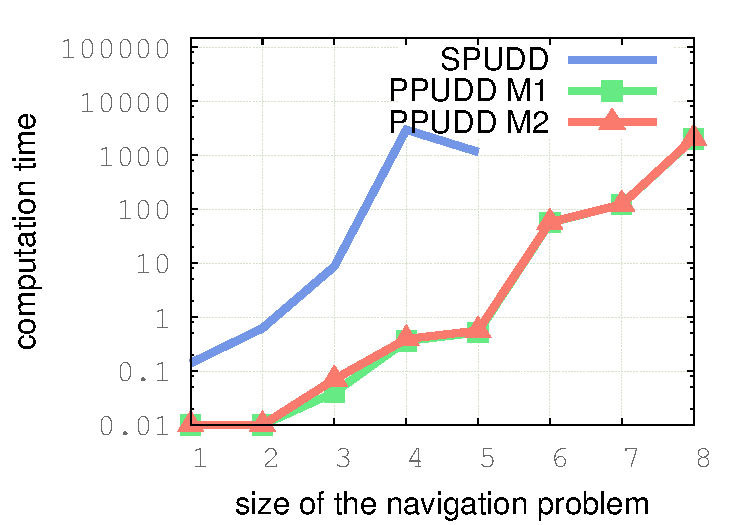
\includegraphics[width=\linewidth]{courbeTime.pdf}
\caption{Computation time (sec)}
\label{navigCT}
\end{subfigure}
\begin{subfigure}[t]{.48\linewidth}
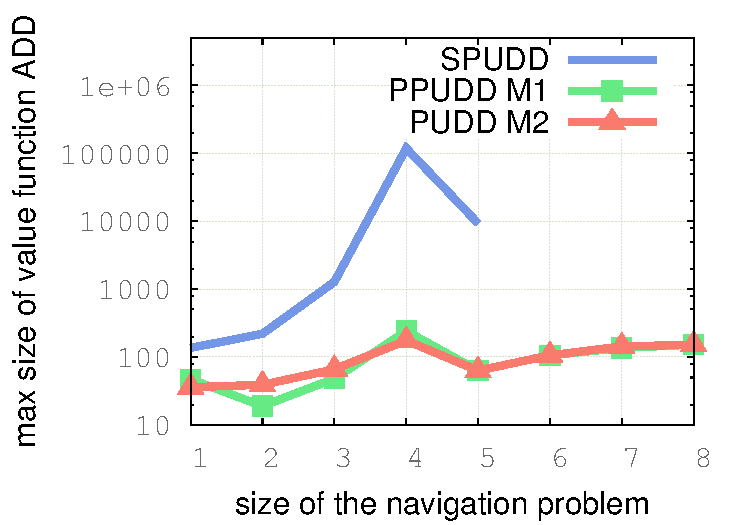
\includegraphics[width=\linewidth]{courbeADD.pdf}
\caption{Size of ADD value function}
\label{navigADD}
\end{subfigure}\\
\vspace{0.5cm}
\begin{subfigure}[b]{.48\linewidth}
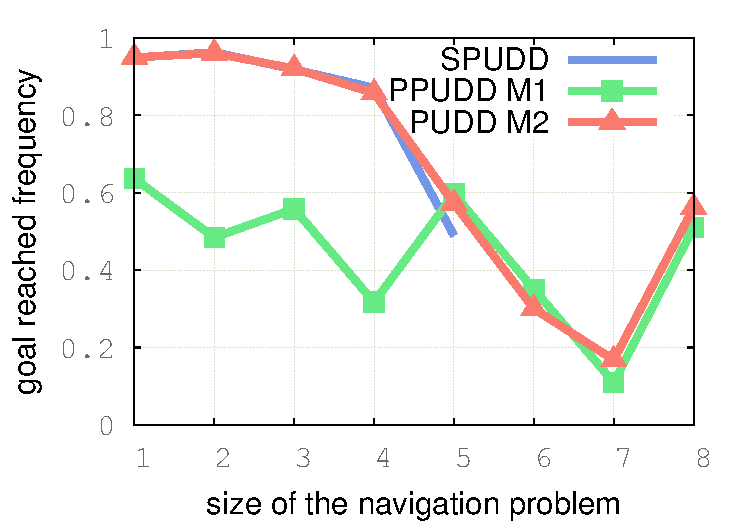
\includegraphics[width=\linewidth]{courbePerfMDP.pdf}
\caption{Reached goal frequency}
\label{navigGOAL}
\end{subfigure}
\begin{subfigure}[b]{.48\linewidth}
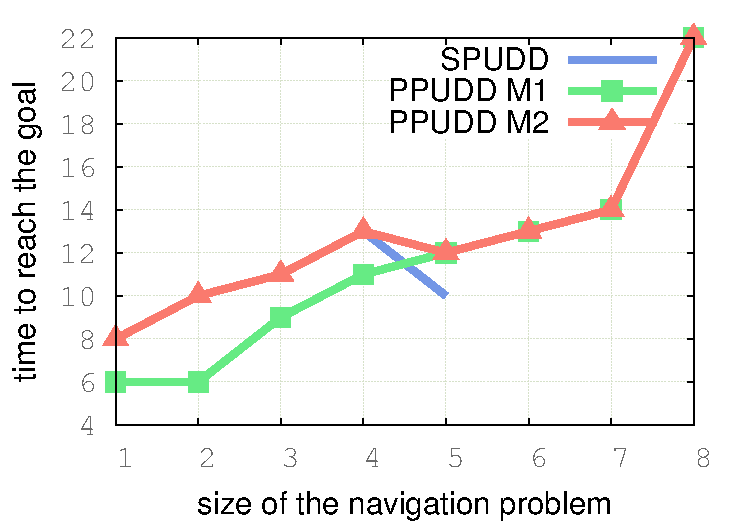
\includegraphics[width=\linewidth]{courbePerfMDP2.pdf}
\caption{Time to reach the goal}
\label{navigL}
\end{subfigure}\\
\vspace{0.5cm}
\caption[PPUDD vs. SPUDD, Navigation problem]{PPUDD vs. SPUDD on the Navigation problem: the $x$-axis represents indexes of problem instances, increasing with the problem sizes.}
\end{figure}
Figure \ref{navigCT} shows that 
SPUDD runs out of memory from the 6$^{\text{th}}$ problem, and PPUDD computation's time
outperforms SPUDD's one by many orders of magnitude for the two models. Intuitively, this result
comes from the fact that PPUDD's ADDs should be smaller because their leaves'
values are in the finite scale $\mathcal{L}$ rather than $\mathbb{R}$, which is indeed
demonstrated in Figure \ref{navigADD}. Performances were evaluated 
with two relevant criteria: frequency of runs where 
the policy reaches the goal (see Figure \ref{navigGOAL}), and
average length of execution runs that reach the goal (see Figure \ref{navigL}), 
that are both functions of the problem's instance.
As expected, model (M2) is more cautious than model (M1) and gets a better 
reached goal frequency  (similar to SPUDD's one for the instances it can solve). 
The later is more optimistic and gets a better average length of execution runs than model (M2) due to
its dangerous behavior. For fairness reasons, we also compared ourselves against 
APRICODD \cite{St-aubin00apricodd:approximate}, 
which is an approximate algorithm for factored MDPs: however parameters impacting the approximation
are hard to tune (either huge computation times, or zero qualities) and it is
largely outperformed by PPUDD in both time and quality whatever the parameters %(figures not shown because APRICODD's 
(curves are not shown since uninformative).\\

Finally, we compared PPUDD on the \textit{Rocksample problem} (RS),
described in Section \ref{section_RS_motivatingEx}, 
against a recent probabilistic MOMDP planner, 
APPL \cite{OngShaoHsuWee-IJRR10}, and a POMDP
planner using ADDs, symbolic HSVI \cite{Sim:2008:SHS:1620163.1620241}. Both
algorithms are approximate and anytime, so we  decided to stop them when they
reached a precision of $1$. 
Figure \ref{figureRS1}, where problem instances
increase with grid size and number of rocks, shows that APPL runs out of memory
at the $8^{th}$ problem instance, symbolic HSVI at the $7^{th}$ one, while PPUDD
outperforms them by many orders of magnitude. 
\begin{figure}\centering
\begin{subfigure}[c]{.48\linewidth}
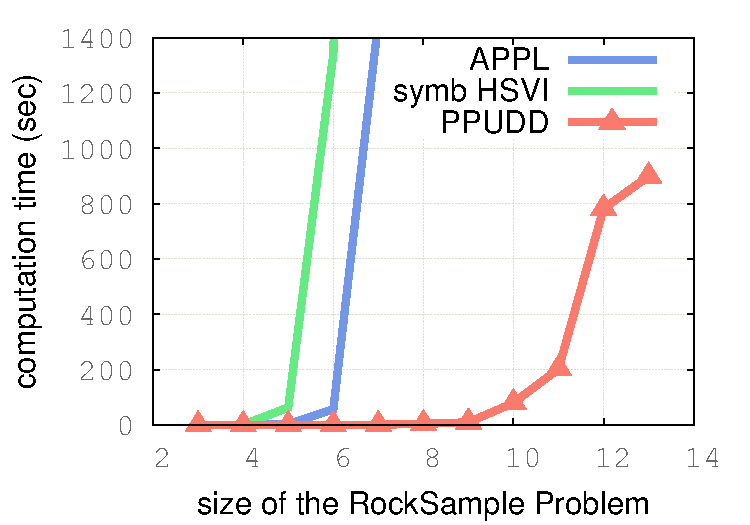
\includegraphics[width=\linewidth]{RockSampleCompTime.pdf}
\caption{Computation time (sec)}
\label{figureRS1}
\end{subfigure}
\begin{subfigure}[c]{.48\linewidth}
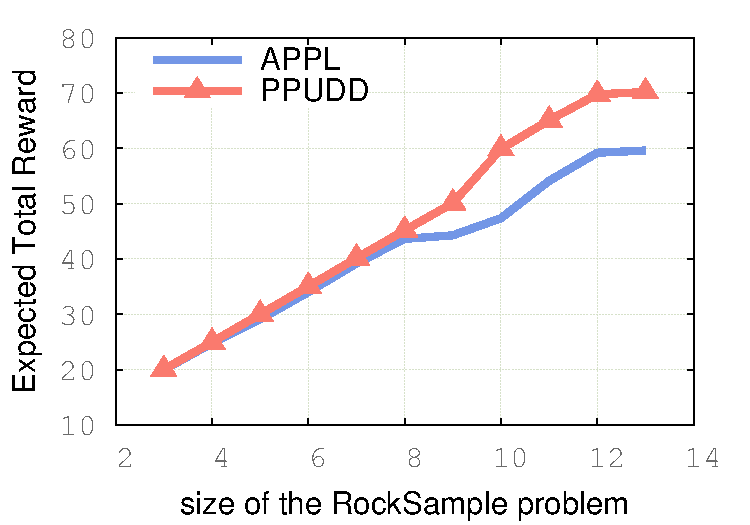
\includegraphics[width=\linewidth]{courbePerfTime.pdf}
\caption{Expected total reward}
\label{figureRS2}
\end{subfigure}
\vspace{0.5cm}
\caption[PPUDD vs. APPL and symb-HSVI, RockSample problem]{PPUDD vs. APPL and symb HSVI on the RockSample problem: the $x$-axis represents indexes of problem instances, increasing with the problem sizes.}
\end{figure}
Instead of precision, computation
time of APPL can be fixed at PPUDD's computation time in order to compare their
expected total rewards (using probabilistic model's rewards) 
after they consumed the same CPU time. 
%For PPUDD, we
%simply evaluated with the probabilistic model the policy that was computed
% under
%possibilistic settings.
Surprisingly, Figure \ref{figureRS2} shows that rewards gathered are higher with
PPUDD than with APPL. The reason is that APPL is in fact an approximate
probabilistic planner, which shows that our approach consisting in exactly
solving an approximate model can outperform algorithms that approximately solve
an exact model. 
Moreover, exact POMDP planners are
unable to scale to problems of the size of the RockSample ones.
Finally, it is worth noting that probabilities of the
observation model, which represent uncertainties of sensor outputs, may be
difficult to precisely know in practice, in which case possibilistic models may
be more physically accurate. 
In fact for this example the policy produced by
PPUDD is the best to get all possible rewards: this is essentially because the
rover can be sure of a rock's nature checking 
when it is on it.

These results assured us that it was not unreasonable to present PPUDD
in the International Probabilistic Planning Competition 2014,
even though the computation of strategies for probabilistic problems 
is not the initial vocation of this solver.
The next section describes the competition context
as well as the presented versions of PPUDD,
and discusses the results of the different competitor solvers.

\subsection{International Probabilistic Planning Competition 2014}
% TODO TODO TODO TODO 
% presentation de la compet 1
% presentation des competiteurs
% presentation de nos versions
% MASK, ATPPUDD, description 
% description des domains et en parallele, les resultats et commentaires
% + citer depot \\

%puis les 2 chaps suivants \\
%puis intro/concl \\


The fully observable track 
of the International Probabilistic Planning Competition (IPPC) 
allows to fairly compare performances of MDP solvers.
The competitors' solvers have to compute 
strategies for some problems 
which are not known in advance.
Given one of these problems, 
solvers have a limited amount of time 
to send actions to the competition server 
which simulates the evolution of the system state:
successive states are sampled by the competition server
using the transition probability 
distributions of the MDP defining the problem, 
and sent to a given competitor's solver.
For each system state received, the solver 
has to send back the action
it has computed.
These data exchanges are conducted 
during few trials of finite horizon and
the score of the solver for the considered problem 
is the average (over trials) 
of the undiscounted and finite sum of 
rewards along the trajectory generated by the trial.

Materials about this competition are available at the official web page of the competition
\url{https://cs.uwaterloo.ca/~mgrzes/IPPC_2014/}.
Problems are grouped in \textit{domains}, 
which are MDPs whose a finite number of parameters are undefined:
the problem, or MDP, used in practice during the competition
is an \textit{instance} of a domain, \textit{i.e.}
a domain whose parameters have been set.
In this competition, $8$ domains have been proposed,
called respectively
\textit{Academic advising}, \textit{Crossing traffic}, \textit{Elevators}, 
\textit{Skill teaching}, \textit{Tamarisk}, \textit{Traffic}, \textit{Triangle tireworld}
and \textit{Wildfire}.
Three possible encodings of the instances of these domains are proposed,
\textit{i.e.} three different languages can be used to describe the instances:
the first is the \textit{Planning Domain Definition Language} (PPDDL, \cite{Younes_ppddl1.0});
the second is a \textit{LISP}-like language introduced with symbolic algorithms such as SPUDD 
which defines explicitely transition probability distributions and reward function as ADDs
(see \url{http://users.cecs.anu.edu.au/~ssanner/IPPC_2011/}); 
finally, the third is the \textit{Relational Dynamic Influence Diagram Language} (RDDL, \cite{Sanner_relationaldynamic})
which is simpler and more expressive than the previous ones.
The competition consists in evaluating the solver over 
$10$ instances per domain with $30$ runs per instance and
$18$ minutes per instance: it takes $24$ hours in total.

In order to ensure that everyone has the same computational power,
each competitor solver is set up in a remote server whose RAM is $7.5$Gb 
with $2$ cores.% (``m3.large'', see \url{https://aws.amazon.com/ec2/pricing/}).
The client and server for the competition are available in the open source \textit{RDDLSim} software, 
which is available online at \url{http://code.google.com/p/rddlsim/}.
Four solvers have been proposed for this competition:
\begin{itemize}
\item \textit{PROST} \cite{DBLP:conf/aips/KellerE12}, based on \textit{Upper Confidence bound applied to Trees} (UCT, \cite{Kocsis:2006:BBM:2091602.2091633})
and using directly RDDL encoding;
\item \textit{GOURMAND} \cite{DBLP:conf/aaai/KolobovMW12,Kolobov12reverseiterative}, based on \textit{Labeled Real Time Dynamic Programming} (LRTDP, \cite{Bonet03labeledrtdp})
using PPDDL encoding;
\item \textit{symbolic LRTDP}, using ADDs and LISP-like encoding \cite{symbLRTDP};
\item our algorithm PPUDD, using LISP-like encoding too.
\end{itemize}

%4 domains from IPPC 2011:
%Traffic Control: highly exogenous, concurrent
%Elevator Control: highly exogenous, concurrent
%Crossing Traffic: goal-oriented, deterministic if move far left
%Skill Teaching: few exogenous events\\

%4 new domains
%Wildfire: from ecological literature, contributed by Zhenyu Yu
%Academic Advising: complex prereq structure, contributed by Libby Ferland
%Tamarisk: from ecological literature, used in 2014 RL Competition
%Triangle Tireworld: probabilistically interesting, from IPPC 2008


%Sum of undiscounted rewards over finite horizon
%Averaged over 30 trials
%server/port (up to 3 if running multiple planners)
%We'll give competitors 24 hours   
%All competitors should use a single EC2 m3.large instance see \url{https://aws.amazon.com/ec2/pricing/},
%(m3.large: vCPU=2, ECU=6.5, Memory (GiB) 7.5, Storage (GB) $1 \times 32$ SSD) 

%Final competition Rules:
%(a) Competition week: The final competition will take place over a one week period where competitors will sign up for a 24 hour time slot during this period.  
%8 competition domains not known in advance: 
%(c) 24 hour Competition slot: The full competition domain and instance 
%list will be released to competitors via a private web link at the start 
%of their chosen 24 hour competition slot.  
%(d) Post-competition: all competitors need to sign a document 
%saying that they have honored the rules above 
%(there will a section to explain any variations, 
%e.g., to list changes on account of debugging).  
%Competitors also need to submit an archive 
%of their source code to the organizers 
%with instructions on how to run the planner 
%to reproduce competition results.  
%(The organizers will not publicly release this code.)  
%(e) Final results: released at ICAPS 2014 
%(June 21-26) and posted to the IPPC website immediately thereafter.

%Planners PPUDD and ATPPUDD are based on the simple idea that
%approximating an MDP with a qualitative model of uncertainty like
%possibilities that still preserves rankings of how likely events may
%occur, can reduce computation complexity without sacrificing too much
%to solution quality. This intuition is emphasized by the observation
%that decision diagrams used in factored MDPs often blow up due to the
%prohibitive number of nodes generated by probabilistic operations.
%Starting with a SPUDD representation of the input problem, PPUDD
%translates transition and reward decision diagrams to possibilistic
%ADDs, then symbolically solves the possibilistic version of Bellman's
%equation. 
%Contrary to SPUDD, 
As the score given to solvers only depends on the $40$ first stages of the process,
the presented version of PPUDD consists of the Algorithm \ref{PPUDD} 
with the ``while condition'' $\overline{U^*} \neq \overline{U^c}$ at line \ref{while_PPUDD}
replaced by the condition ``iteration $\leqslant 40$''.
It also incrementally augments the planning
horizon while maintaining a mask stored in form of 
a Binary Decision Diagram (BDD, \textit{i.e.} an ADD with leaves in $\set{0,1}$) 
representing the states reachable from the initial state:
the computation of the current value function is then restricted
to the reachable states only. While PPUDD is an offline algorithm,
we proposed also \textit{AnyTime PPUDD} (ATPPUDD) 
which is an anytime version which learns computation times of
Bellman backups while dispatching the computational effort accordingly
over the remaining planning horizon much like GOURMAND does in the
probabilistic world (see \cite{DBLP:conf/aaai/KolobovMW12}). 

When encoded with the LISP-like format, 
problems of the competition, \textit{i.e.} instances of each domains, 
are described as factored MDPs
with boolean system state variables: 
for each action $a \in \mathcal{A}$ and for each next boolean system state variable $X_i'$, 
one ADD representing the corresponding transition probability distribution
$\textbf{p} \Big( X_i' \ \Big\vert \ parents(X_i'), a \Big)$ is given.
In order to define the $\pi$-MDP which will be solved by PPUDD,
we simply normalize these distributions in the possibilistic sense:
we set to $1$ the possibility degree of an assignment of $X_i'$ when 
its probability value is maximal, and to the probability value otherwise.
For instance, for a given assignment of the previous variables $parents(X_i')$, 
if the probability value of the assignment (or event) $X_i'=1$ is $0.7$ 
(and thus probability $0.3$ that $X_i' = 0$), 
then the possibility degree of $X_i'=1$ is set to $1$,
and the one of $X_i' = 0$ is set to $0.3$.

In terms of ADDs, it can be computed as follows:
let us first recall the notation  $\textbf{p} \Big( X_i' \ \Big\vert \ parents(X_i'),a \Big)^{X_i'=0}$,
used to represent the subtree of the ADD
$\textbf{p} \Big( X_i' \ \Big\vert \ parents(X_i'),a \Big)$ setting $X_i'$ to false (\textit{i.e.} to $0$).
As well, $\textbf{p} \Big( X_i' \ \Big\vert \ parents(X_i'),a \Big)^{X_i'=1}$ is the subtree of the same ADD, setting $X_i'$ to true (\textit{i.e.} to $1$).
Let us denote by $\mathds{1}_{\textbf{p}_{\top}>\textbf{p}_{\bot}}$ 
the BDD equal to $1$ for each variable assignment such that %$X_i'$ is true ($X_i'=\top$),
%and $0$ otherwise. 
%for each assignment of the variables of $parents(X_i')$ such that 
%\ovalbox{$\min$}
\[ \textbf{p} \Big( X_i' \ \Big\vert \ parents(X_i'),a \Big)^{X_i'=0} < \textbf{p} \Big( X_i' \ \Big\vert \ parents(X_i'),a \Big)^{X_i'=1}, \]
and equal to $0$ for other assignments.
The BDD always equal to $1$ is denoted by $\mathds{1}$. 
The BDD $\mathds{1}_{\textbf{p}=0.5}$ is equal to $1$
for variable assignments such that the probability of the event $X_i'=1$ (or $X_i'=0$) 
is equal to $0.5$, and this BDD is equal to $0$ otherwise.
We can also denote by
$\mathds{1}_{\textbf{p}_{\top}<\textbf{p}_{\bot}} $
the BDD which is equal to $1$ for assignments of variables in $parents(X_i')$ 
such that the probability of event $X_i' = 1$
is lower than the probability of event $X_i'=0$:
this BDD can be computed from previous BDDs,
$ \mathds{1} \ \ovalbox{$-$} \ \mathds{1}_{\textbf{p}_{\top}>\textbf{p}_{\bot}} \ \ovalbox{$-$} \ \mathds{1}_{\textbf{p}=0.5}$,
where $\ovalbox{$-$}$ is the minus operator, applied to trees.
The possibility transition distribution for the $i^{th}$ variable is
\begin{eqnarray*}
\pi \Big( X_i' \ \Big\vert \ parents(X_i'),a \Big) = \ovalbox{$\max$} \Bigg\{ 	& \mathds{1}_{\textbf{p}=0.5}, 														& \\
				& \ovalbox{$\min$} \bigg\{ \mathds{1}_{\textbf{p}_{\top}>\textbf{p}_{\bot}}, \textbf{p} \Big( X_i' \Big\vert parents(X_i'), a \Big) \bigg\} , 	& \\
				& \ovalbox{$\min$} \bigg\{ \mathds{1}_{\textbf{p}_{\top}<\textbf{p}_{\bot}}  , \textbf{p} \Big( X_i' \Big\vert parents(X_i'), a \Big) \bigg\} 	& 	\Bigg\} 
\end{eqnarray*}

As well, for each action $a \in \mathcal{A}$, 
an ADD representing the reward function for this action 
is provided and denoted by $r(X_1,\ldots,X_n,a)$. 
Let us define then for each $s \in \mathcal{S}$ and $a \in \mathcal{A}$,
\[ \Psi(s,a) = \frac{ r(s,a) - \min_{s,a} r(s,a) }{ \max_{s,a} r(s,a) - \min_{s,a} r(s,a)} \in [0,1]. \]
The terminal preference function is set to $\Psi(s) = \max_{a \in \mathcal{A}} \Psi(s,a)$,
and the strategy is initialized by $\delta^*(s) \in \operatorname*{argmax}_{a \in \mathcal{A}} \Psi(s,a)$
at the beginning of the algorithm.

Note that possibility and preference degrees are not in a scale $\mathcal{L}$ 
as previously defined (\textit{i.e.} $\set{ 0, \frac{1}{k}, \frac{2}{k} \ldots, 1 }$ for some $k \geqslant1$).
Indeed, possibility degrees comes from probability values, 
and preferences are normalized rewards.
However, only $\max$ and $\min$ operators are used, 
so it has no impact on the qualitative results of the computations. 

The library used to perform computations with ADDs
is the \textit{CU Decision Diagram Package} 
(CUDD, \url{http://vlsi.colorado.edu/~fabio/CUDD/}),
and the described versions of PPUDD are available 
at the adress \url{https://github.com/drougui/ppudd}.

Following figures illustrates the results of IPPC 2014:
the score is given in function of the instance index,
which generally increases with the difficulty (or the size) 
of the associated problem.

\begin{figure} \centering
\definecolor{ggreen}{rgb}{0.3,0.7,0.4}
\begin{tikzpicture}
\begin{axis}[grid=major,xmin=1,xmax=10,xtick={1,2,3,4,5,6,7,8,9,10},
legend entries={GOURMAND, PROST, Symbolic LRTDP, random strategy, ``noop'' strategy, ATPPUDD, PPUDD},legend style={at={(1.52,1.1)}},
xlabel={Problem instances},
ylabel={Raw average score},
title={\textit{Academic advising} problem},width=11cm,height=11cm]
\addplot+[line width=1pt] plot[error bars/.cd,y dir=both,y explicit] table[x index=1, y index=5, y error index=6]{IPPC14_resultats/academic_advising.txt};%GOURMAND
\addplot+[line width=1pt] plot[error bars/.cd,y dir=both,y explicit] table[x index=1, y index=26, y error index=27]{IPPC14_resultats/academic_advising.txt};%PROST14
\addplot+[line width=1pt] plot[error bars/.cd,y dir=both,y explicit] table[x index=1, y index=40, y error index=41]{IPPC14_resultats/academic_advising.txt};%FACTOREDLRTDP
\addplot+[line width=1pt] plot[error bars/.cd,y dir=both,y explicit] table[x index=1, y index=33, y error index=34]{IPPC14_resultats/academic_advising.txt};%RANDOM
\addplot+[color=black,line width=1pt] plot[error bars/.cd,y dir=both,y explicit] table[x index=1, y index=12, y error index=13]{IPPC14_resultats/academic_advising.txt};%NOOP
\addplot[color=ggreen,mark=diamond,line width=3.2pt] plot[error bars/.cd,y dir=both,y explicit] table[x index=1, y index=54, y error index=55]{IPPC14_resultats/academic_advising.txt};%ATPPUDD 
\addplot[color=orange,mark=diamond,line width=2.2pt] plot[error bars/.cd,y dir=both,y explicit] table[x index=1, y index=47, y error index=48]{IPPC14_resultats/academic_advising.txt};%PPUDD 
\end{axis}
\end{tikzpicture}
\\
\vspace{0.5cm}
\begin{tikzpicture}
\begin{axis}[grid=major,xmin=1,xmax=10,xtick={1,2,3,4,5,6,7,8,9,10},
xlabel={Problem instances},
ylabel={Raw average score},
title={\textit{Crossing traffic} problem},width=11cm,height=11cm]
\addplot+[line width=1pt] plot[error bars/.cd,y dir=both,y explicit] table[x index=1, y index=5, y error index=6]{IPPC14_resultats/crossing_traffic_inst_mdp.txt};%GOURMAND
\addplot+[line width=1pt] plot[error bars/.cd,y dir=both,y explicit] table[x index=1, y index=26, y error index=27]{IPPC14_resultats/crossing_traffic_inst_mdp.txt};%PROST14
\addplot+[line width=1pt] plot[error bars/.cd,y dir=both,y explicit] table[x index=1, y index=40, y error index=41]{IPPC14_resultats/crossing_traffic_inst_mdp.txt};%FACTOREDLRTDP
\addplot+[line width=1pt] plot[error bars/.cd,y dir=both,y explicit] table[x index=1, y index=33, y error index=34]{IPPC14_resultats/crossing_traffic_inst_mdp.txt};%RANDOM
\addplot+[color=black,line width=1pt] plot[error bars/.cd,y dir=both,y explicit] table[x index=1, y index=12, y error index=13]{IPPC14_resultats/crossing_traffic_inst_mdp.txt};%NOOP
\addplot[color=ggreen,mark=diamond,line width=3.2pt] plot[error bars/.cd,y dir=both,y explicit] table[x index=1, y index=54, y error index=55]{IPPC14_resultats/crossing_traffic_inst_mdp.txt};%ATPPUDD 
\addplot[color=orange,mark=diamond,line width=2.2pt] plot[error bars/.cd,y dir=both,y explicit] table[x index=1, y index=47, y error index=48]{IPPC14_resultats/crossing_traffic_inst_mdp.txt};%PPUDD 
\end{axis}
\end{tikzpicture}
\caption[Results of IPPC 2014: \textit{Academic advising} and \textit{Crossing traffic} problems]{
Results of the International Probabilistic Planning Competition -- Fully Observable track}
\label{figure_IPPC_ACA_CRO}
\end{figure}

Figure \ref{figure_IPPC_ACA_CRO} presents the scores obtained by each solver 
for each of the $10$ instances of the \textit{Academic advising} domains,
\textit{i.e.} the average over $30$ trials of the sum of the encountered rewards.
Performances of our algorithms are close to the best ones.
However, an unexplained and unwanted bug occurred with ATPPUDD for the $2^{nd}$ instance, 
as only $3$ runs have been performed by this solver.
For the other instances, PPUDD and ATPPUDD produce strategies with performances like 
PROST and GOURMAND, and better than Symbolic LRTDP.
This has been less true for the \textit{Crossing traffic} problem, 
whose results are also described by Figure \ref{figure_IPPC_ACA_CRO}.
This problem models a robot which has to reach a goal 
which is across an highway with a lot of cars.
These cars arrive randomly and move left.
As the possibility degree of the fact that no car arrive 
is set to $1$ by our naive MDP to $\pi$-MDP translation,
the optimistic criterion leads to decide to cross the street,
even if an unseen car may arrive (with a probability $<0.5$ but bit enough to be cautious). 
This explain the poor quality of the produced strategies 
for this domain. Note however that, for the $6$ last instances (most difficult problems)
our approach leads to better strategies than the probabilistic solver Symbolic LRTDP.

\begin{figure} \centering
\definecolor{ggreen}{rgb}{0.3,0.7,0.4}
\begin{tikzpicture}
\begin{axis}[grid=major,xmin=1,xmax=10,xtick={1,2,3,4,5,6,7,8,9,10},
legend entries={GOURMAND, PROST, Symbolic LRTDP, random strategy, ``noop'' strategy, ATPPUDD, PPUDD},legend style={at={(1.52,1.1)}},width=11cm,height=11cm,
xlabel={Problem instances},
ylabel={Raw average score},
title={\textit{Elevators} problem}]
\addplot+[line width=1pt] plot[error bars/.cd,y dir=both,y explicit] table[x index=1, y index=5, y error index=6]{IPPC14_resultats/elevators_inst_mdp.txt};%GOURMAND
\addplot+[line width=1pt] plot[error bars/.cd,y dir=both,y explicit] table[x index=1, y index=26, y error index=27]{IPPC14_resultats/elevators_inst_mdp.txt};%PROST14
\addplot+[line width=1pt] plot[error bars/.cd,y dir=both,y explicit] table[x index=1, y index=40, y error index=41]{IPPC14_resultats/elevators_inst_mdp.txt};%FACTOREDLRTDP
\addplot+[line width=1pt] plot[error bars/.cd,y dir=both,y explicit] table[x index=1, y index=33, y error index=34]{IPPC14_resultats/elevators_inst_mdp.txt};%RANDOM
\addplot+[color=black,line width=1pt] plot[error bars/.cd,y dir=both,y explicit] table[x index=1, y index=12, y error index=13]{IPPC14_resultats/elevators_inst_mdp.txt};%NOOP
\addplot[color=ggreen,mark=diamond,line width=3.2pt] plot[error bars/.cd,y dir=both,y explicit] table[x index=1, y index=54, y error index=55]{IPPC14_resultats/elevators_inst_mdp.txt};%ATPPUDD 
\addplot[color=orange,mark=diamond,line width=2.2pt] plot[error bars/.cd,y dir=both,y explicit] table[x index=1, y index=47, y error index=48]{IPPC14_resultats/elevators_inst_mdp.txt};%PPUDD 
\end{axis}
\end{tikzpicture}
\\
\vspace{0.5cm}
\begin{tikzpicture}
\begin{axis}[grid=major,xmin=1,xmax=10,xtick={1,2,3,4,5,6,7,8,9,10},
xlabel={Problem instances},
ylabel={Raw average score},
title={\textit{Skill teaching} problem},width=11cm,height=11cm]
\addplot+[line width=1pt] plot[error bars/.cd,y dir=both,y explicit] table[x index=1, y index=5, y error index=6]{IPPC14_resultats/skill_teaching_inst_mdp.txt};%GOURMAND
\addplot+[line width=1pt] plot[error bars/.cd,y dir=both,y explicit] table[x index=1, y index=26, y error index=27]{IPPC14_resultats/skill_teaching_inst_mdp.txt};%PROST14
\addplot+[line width=1pt] plot[error bars/.cd,y dir=both,y explicit] table[x index=1, y index=40, y error index=41]{IPPC14_resultats/skill_teaching_inst_mdp.txt};%FACTOREDLRTDP
\addplot+[line width=1pt] plot[error bars/.cd,y dir=both,y explicit] table[x index=1, y index=33, y error index=34]{IPPC14_resultats/skill_teaching_inst_mdp.txt};%RANDOM
\addplot+[color=black,line width=1pt] plot[error bars/.cd,y dir=both,y explicit] table[x index=1, y index=12, y error index=13]{IPPC14_resultats/skill_teaching_inst_mdp.txt};%NOOP
\addplot[color=ggreen,mark=diamond,line width=3.2pt] plot[error bars/.cd,y dir=both,y explicit] table[x index=1, y index=54, y error index=55]{IPPC14_resultats/skill_teaching_inst_mdp.txt};%ATPPUDD 
\addplot[color=orange,mark=diamond,line width=2.2pt] plot[error bars/.cd,y dir=both,y explicit] table[x index=1, y index=47, y error index=48]{IPPC14_resultats/skill_teaching_inst_mdp.txt};%PPUDD 
\end{axis}
\end{tikzpicture}
\caption[Results of IPPC 2014: \textit{Elevators} and \textit{Skill teaching problems}]{
Results of the International Probabilistic Planning Competition -- Fully Observable track}
\label{figure_IPPC_ELE_SKI}
\end{figure}

In the \textit{Elevators} problem, people arrive randomly and have to be transported 
to the correct building stage: 
as the frequentist information is lost using the possibilistic approach
and seems important in this problem (people do not want to wait once arrived), 
scores of our algorithms are poorer than the ones of PROST and GOURMAND.
The toy example at the beginning of the introduction of this chapter
illustrates that the possibilistic approaches can select actions probabilistically clearly suboptimal
when the probability values are at the heart of the problem.
PPUDD and ATPPUDD are however better than Symbolic LRTDP, as shown by Figure \ref{figure_IPPC_ELE_SKI},
and than doing nothing (``noop strategy'') or choosing actions randomly (``random strategy'').
PPUDD and ATPPUDD have quite good behaviours with the \textit{Skill teaching} problem 
as illustrated by the same figure. Moreover, ATPPUDD leads to better results
for the last three instances: as these instances are the \textit{Skill teaching} problems 
with the largest system space,  
the anytime version, which manages the computation time, 
produces strategies with better performances
than PPUDD, which classically solve the associated $\pi$-MDP, 
but cannot complete computations and lead to a poorer strategy.

\begin{figure} \centering
\definecolor{ggreen}{rgb}{0.3,0.7,0.4}
\begin{tikzpicture}
\begin{axis}[grid=major,xmin=1,xmax=10,xtick={1,2,3,4,5,6,7,8,9,10},
xlabel={Problem instances},
ylabel={Raw average score},
title={\textit{Tamarisk} problem},
compat=newest,
legend entries={GOURMAND, PROST, Symbolic LRTDP, random strategy, ``noop'' strategy, ATPPUDD, PPUDD},legend style={at={(1.52,1.1)}},width=11cm,height=11cm]
\addplot+[line width=1pt] plot[error bars/.cd,y dir=both,y explicit] table[x index=1, y index=5, y error index=6]{IPPC14_resultats/tamarisk.txt};%GOURMAND
\addplot+[line width=1pt] plot[error bars/.cd,y dir=both,y explicit] table[x index=1, y index=26, y error index=27]{IPPC14_resultats/tamarisk.txt};%PROST14
\addplot+[line width=1pt] plot[error bars/.cd,y dir=both,y explicit] table[x index=1, y index=40, y error index=41]{IPPC14_resultats/tamarisk.txt};%FACTOREDLRTDP
\addplot+[line width=1pt] plot[error bars/.cd,y dir=both,y explicit] table[x index=1, y index=33, y error index=34]{IPPC14_resultats/tamarisk.txt};%RANDOM
\addplot+[color=black,line width=1pt] plot[error bars/.cd,y dir=both,y explicit] table[x index=1, y index=12, y error index=13]{IPPC14_resultats/tamarisk.txt};%NOOP
\addplot[color=ggreen,mark=diamond,line width=3.2pt] plot[error bars/.cd,y dir=both,y explicit] table[x index=1, y index=54, y error index=55]{IPPC14_resultats/tamarisk.txt};%ATPPUDD 
\addplot[color=orange,mark=diamond,line width=2.2pt] plot[error bars/.cd,y dir=both,y explicit] table[x index=1, y index=47, y error index=48]{IPPC14_resultats/tamarisk.txt};%PPUDD 
\end{axis}
\end{tikzpicture}
\\
\vspace{0.5cm}
\begin{tikzpicture}
\begin{axis}[grid=major,xmin=1,xmax=10,xtick={1,2,3,4,5,6,7,8,9,10},
xlabel={Problem instances},
ylabel={Raw average score},
title={\textit{Traffic} problem},
width=11cm,height=11cm]
\addplot+[line width=1pt] plot[error bars/.cd,y dir=both,y explicit] table[x index=1, y index=5, y error index=6]{IPPC14_resultats/traffic_inst_mdp.txt};%GOURMAND
\addplot+[line width=1pt] plot[error bars/.cd,y dir=both,y explicit] table[x index=1, y index=26, y error index=27]{IPPC14_resultats/traffic_inst_mdp.txt};%PROST14
\addplot+[line width=1pt] plot[error bars/.cd,y dir=both,y explicit] table[x index=1, y index=40, y error index=41]{IPPC14_resultats/traffic_inst_mdp.txt};%FACTOREDLRTDP
\addplot+[line width=1pt] plot[error bars/.cd,y dir=both,y explicit] table[x index=1, y index=33, y error index=34]{IPPC14_resultats/traffic_inst_mdp.txt};%RANDOM
\addplot+[color=black,line width=1pt] plot[error bars/.cd,y dir=both,y explicit] table[x index=1, y index=12, y error index=13]{IPPC14_resultats/traffic_inst_mdp.txt};%NOOP
\addplot[color=ggreen,mark=diamond,line width=3.2pt] plot[error bars/.cd,y dir=both,y explicit] table[x index=1, y index=54, y error index=55]{IPPC14_resultats/traffic_inst_mdp.txt};%ATPPUDD 
\addplot[color=orange,mark=diamond,line width=2.2pt] plot[error bars/.cd,y dir=both,y explicit] table[x index=1, y index=47, y error index=48]{IPPC14_resultats/traffic_inst_mdp.txt};%PPUDD 
\end{axis}
\end{tikzpicture}
\caption[Results of IPPC 2014: \textit{Tamarisk} and \textit{Traffic} problems]{
Results of the International Probabilistic Planning Competition -- Fully Observable track}
\label{figure_IPPC_TAM_TRA}
\end{figure}


With respect to other solvers, possibilistic solvers have good results 
with the \textit{Tamarisk} domain, as shown in Figure \ref{figure_IPPC_TAM_TRA}..
However, some instances (e.g. the $6^{th}$, the $8^{th}$ and the $10^{th}$) 
are not even run as the ADD instantiation takes too long. 
Symbolic LRTP faces the same issue
as it uses also the LISP-like encoding of the problem.
We think that this is an issue specific to the competition,
as each problem has to be equivalently translated into
three different languages (RDDL, PPDDL and LISP-like),
which produces sometimes artificially complex
encodings of the problems.
The \textit{Traffic} domain is really hard to solve by PPUDD and ATPPUDD (see Figure \ref{figure_IPPC_TAM_TRA}). 
Actually the least scores are obtained with this domain,
and even the random and the noop strategies are better strategies.
Note that we did not implement any ``watchdog''
returning random actions when the computed strategy is less effective than the random one.
However, this kind of gadget is essential to improve results for such large and risky problem. 
As mentioned above for the \textit{Crossing traffic} problem, 
the optimistic criterion may lead to dangerous actions, as it does here.
Moreover, as this problem involves frequentist information (car arrivals)
an high suboptimality of the strategy produced by the possibilistic approach
is confirmed for this kind of problems (see the \textit{Elevator} problems). 
Finally, the \textit{Traffic} problem is known to be one of the hardest domain,
so ADD instantiation takes long, as well as computations, 
which are then not proceeded enough to produce satisfying results. 

\begin{figure} \centering
\definecolor{ggreen}{rgb}{0.3,0.7,0.4}
\begin{tikzpicture}
\begin{axis}[grid=major,xmin=1,xmax=10,xtick={1,2,3,4,5,6,7,8,9,10},
legend entries={GOURMAND, PROST, Symbolic LRTDP, random strategy, ``noop'' strategy, ATPPUDD, PPUDD},legend style={at={(1.52,1.1)}},width=11cm,height=11cm,
xlabel={Problem instances},
ylabel={Raw average score},
title={\textit{Triangle tireworld} problem}]
\addplot+[line width=1pt] plot[error bars/.cd,y dir=both,y explicit] table[x index=1, y index=5, y error index=6]{IPPC14_resultats/triangle_tireworld_inst_mdp.txt};%GOURMAND
\addplot+[line width=1pt] plot[error bars/.cd,y dir=both,y explicit] table[x index=1, y index=26, y error index=27]{IPPC14_resultats/triangle_tireworld_inst_mdp.txt};%PROST14
\addplot+[line width=1pt] plot[error bars/.cd,y dir=both,y explicit] table[x index=1, y index=40, y error index=41]{IPPC14_resultats/triangle_tireworld_inst_mdp.txt};%FACTOREDLRTDP
\addplot+[line width=1pt] plot[error bars/.cd,y dir=both,y explicit] table[x index=1, y index=33, y error index=34]{IPPC14_resultats/triangle_tireworld_inst_mdp.txt};%RANDOM
\addplot+[color=black,line width=1pt] plot[error bars/.cd,y dir=both,y explicit] table[x index=1, y index=12, y error index=13]{IPPC14_resultats/triangle_tireworld_inst_mdp.txt};%NOOP
\addplot[color=ggreen,mark=diamond,line width=3.2pt] plot[error bars/.cd,y dir=both,y explicit] table[x index=1, y index=54, y error index=55]{IPPC14_resultats/triangle_tireworld_inst_mdp.txt};%ATPPUDD 
\addplot[color=orange,mark=diamond,line width=2.2pt] plot[error bars/.cd,y dir=both,y explicit] table[x index=1, y index=47, y error index=48]{IPPC14_resultats/triangle_tireworld_inst_mdp.txt};%PPUDD
\end{axis}
\end{tikzpicture}
\\
\vspace{0.5cm}
\begin{tikzpicture}
\begin{axis}[grid=major,xmin=1,xmax=10,xtick={1,2,3,4,5,6,7,8,9,10}, width=11cm,height=11cm,
xlabel={Problem instances},
ylabel={Raw average score},
title={\textit{Wildfire} problem}]
\addplot+[line width=1pt] plot[error bars/.cd,y dir=both,y explicit] table[x index=1, y index=5, y error index=6]{IPPC14_resultats/wildfire_inst_mdp.txt};%GOURMAND
\addplot+[line width=1pt] plot[error bars/.cd,y dir=both,y explicit] table[x index=1, y index=26, y error index=27]{IPPC14_resultats/wildfire_inst_mdp.txt};%PROST14
\addplot+[line width=1pt] plot[error bars/.cd,y dir=both,y explicit] table[x index=1, y index=40, y error index=41]{IPPC14_resultats/wildfire_inst_mdp.txt};%FACTOREDLRTDP
\addplot+[line width=1pt] plot[error bars/.cd,y dir=both,y explicit] table[x index=1, y index=33, y error index=34]{IPPC14_resultats/wildfire_inst_mdp.txt};%RANDOM
\addplot+[color=black,line width=1pt] plot[error bars/.cd,y dir=both,y explicit] table[x index=1, y index=12, y error index=13]{IPPC14_resultats/wildfire_inst_mdp.txt};%NOOP
\addplot[color=ggreen,mark=diamond,line width=3.2pt] plot[error bars/.cd,y dir=both,y explicit] table[x index=1, y index=54, y error index=55]{IPPC14_resultats/wildfire_inst_mdp.txt};%ATPPUDD 
\addplot[color=orange,mark=diamond,line width=2.2pt] plot[error bars/.cd,y dir=both,y explicit] table[x index=1, y index=47, y error index=48]{IPPC14_resultats/wildfire_inst_mdp.txt};%PPUDD 
\end{axis}
\end{tikzpicture}
\caption[Results of IPPC 2014: \textit{Triangle tireworld} and \textit{Wildfire} problems]{
Results of the International Probabilistic Planning Competition -- Fully Observable track}
\label{figure_IPPC_TRI_WIL}
\end{figure}

Finally, the two last domains, whose results are described in Figure \ref{figure_IPPC_TRI_WIL},
are called \textit{Triangle Tireworld} and \textit{Wildfire}.
Firt, ATPPUDD faces an unexplained bug for each instance of the \textit{Triangle Tireworld} domain:
no trial is performed from the $5^{th}$ instance, and maximum $2$ trials are performed for other instances
(which explains the poor score for each instance).
As already mentioned for the \textit{Tamarisk} domain, 
ADD instantiation takes too long for the last instances,
and no trial is performed for the last $4$ instances 
with PPUDD too: Symbolic LRTDP faces the same issue. 
The last domain, called \textit{Wildfire}, leads to highly frequentist problems:
it involves random fire starts. 
That is why PPUDD and ATPPUDD strategies are not really efficient, 
but not too distant from Symbolic LRTDP solver's results.

%%%% TODO TODO TODO TODO TODO TODO TODO TODO TODO TODO TODO TODO
%%%% TODO TODO TODO TODO TODO TODO TODO TODO TODO TODO TODO TODO
%%%% TODO TODO TODO TODO TODO TODO TODO TODO TODO TODO TODO TODO
%%%% TODO TODO TODO TODO TODO TODO TODO TODO TODO TODO TODO TODO
%\section{Practical Implementation of the Algorithms using ADDs}
%CUDD library
%%%% TODO TODO TODO TODO TODO TODO TODO TODO TODO TODO TODO TODO
%%%% TODO TODO TODO TODO TODO TODO TODO TODO TODO TODO TODO TODO
%%%% TODO TODO TODO TODO TODO TODO TODO TODO TODO TODO TODO TODO
%%%% TODO TODO TODO TODO TODO TODO TODO TODO TODO TODO TODO TODO


\section{Conclusion} 
We presented PPUDD, the first algorithm to the best of our knowledge that 
solves factored possibilistic qualitative (MO)MDPs with symbolic calculations. In our opinion,
possibilistic models are a good tradeoff between non-deterministic ones, whose
uncertainties are not at all quantified yielding a very approximate model, and
probabilistic ones, where uncertainties are fully specified,
sometimes arbitrarily in practice. Moreover,
$\pi$-MOMDPs reason about finite values in a qualitative scale $\mathcal{L}$ whereas
probabilistic MOMDPs deal with values in $\mathbb{R}$, which implies larger ADDs
for symbolic algorithms. Also, the former reduce to finite-state belief
$\pi$-MDPs contrary to the latter that yield \emph{continuous}-state belief MDPs
of significantly higher complexity. Our experimental results highlight the point that using an
exact algorithm (PPUDD) for an approximate model ($\pi$-MDPs) can bring significantly faster computations
than reasoning about complex exact models, while providing better
strategies than approximate algorithms (APPL) for exact models. 
In the future, we would like to developp a probabilistic algorithm using 
the generalization of our possibilistic belief factorization theory to
probabilistic settings (see Theorem \ref{thm_factoredPROBbelief}): 
related but sightly different results have been proposed for
probabilistic POMDPs \cite{DBLP:conf/aips/ShaniPBS08}. 
These results also does not concern 
the case of mixed observability.

This chapter finally presents the results of our possibilistic approach
during IPPC 2014: 
the highlighted bottleneck of our possibilistic algorithms
resides on the translation from probabilities to possibilities: 
the naive automated translation presented before the description of the results 
leads to poor policies in benchmarks with complex dynamics and reward structures.
Another issue is the size of the input LISP-like encoded domains whose ADD
instantiation before optimization takes a very long time or 
does not even fit into memory for many difficult benchmarks:
this difficulty is shared with the Symbolic LRTDP solver.
However, there is almost no discretization of the initial probability values defining the MDP
in order to produce the possibility degrees
during the instantiation of the ADD defining the $\pi$-MDP:
the maximal difference between two possibility degrees is set to $10^{-3}$.
Stronger discretizations have not been tested yet, 
and could improve scores of our solvers for problems with such memory issues.
Modeling issues have been also highlighted, 
namely the fact that some problems request 
a cautious behaviour, not provided by the use of
the optimistic criterion (see Definition \ref{probstylerewrittenMOMDPcrit}) 
used during the competition. 
Moreover, as illustrated in introduction, 
these experiments show that problems with high entropy events 
are outperformed by probabilistic approaches since the possibilistic 
approach does not take into account the frequentist information about the problem.
The use of \textit{lexi}-approaches, as used in the following chapter, 
may be a possibilistic stratagem to get around this issue.
Note finally that the partially observable version of PPUDD 
(with the generation of a mask of reachable belief states, avoiding useless computations
on unreachable beliefs) is also available on the repository \url{https://github.com/drougui/ppudd}.

The next chapter, Chapter \ref{chap_IHM}, deals with \textit{Human-Machine Interaction} (HMI)
problems: the uncertainty dynamics of the system are in this context typically not known in terms
of probability values, and the qualitative possibilistic approach is shown to be a natural approach
to produce efficient diagnosis of human errors.

Finally, the last chapter, Chapter \ref{chap_hybrid},
takes into account the remarks made using the results of IPPC14:
an approach using Probability and Possibility Theory
in order to benefit from both approaches in the resolution of factored POMDPs
is presented: quantitative information of the problem is kept to avoid the highlighted modeling issues,
and the belief state is handled in a possibilistic way, in order to get a smart discretization of it
and to benefit from a finite and factorized belief state spaces.
This approach leads to a factored probabilistic MDP 
which can be solved for instance by GOURMAND or PROST
(which does not use the memory constraining LISP-like encoding).


\vide{
\subsection{Factored POMDPs -- RDDL}
\begin{itemize}
\item introduction des $\pi$-MDP factoris\'es \\
\textit{car ils permettent la r\'esolution de gros probl\`emes totallement observables}
\item factorization du cas partiellement observable (Pearl,BenAmor) \\
\textit{car ils permettent la r\'esolution de certain probl\`emes totallement observables}
\item approche symbolique, fully observable, CUDD (ADDs):  PPUDD -- IPPC \\
\textit{car ils mettent en place les calculs pour une r\'esolution \'econome en temps de calculs, et tr\`es adapt\'es aux possibilit\'ees qualitatives}
\item algorithme pour le cas partiellement observable \\
\textit{car il g\'en\'eralise l'algorithme du cas totallement observable}
\item observation des limites du qualitatif et du symbolique
\end{itemize}
}

